Cette section va établir que, relativement au problème d'isopérimétrie polygonal,
un \ngone\ solution doit être convexe, 
puis
qu'un \ngone\ convexe solution doit être un \nreg,
et enfin
que si $\setproba*{R}{1}$ et $\setproba*{R}{2}$ sont respectivement un \xgone{k_1} et un \xgone{k_2}, tous les deux réguliers convexes, avec 
$k_1 < k_2$ et $\perim{\setproba*{R}{1}} = \perim{\setproba*{R}{2}}$, 
alors
$\area{\setproba*{R}{1}} < \area{\setproba*{R}{2}}$.
Nous pourrons alors conclure dans la section finale suivante.


\begin{tcolorbox}
	\itshape\small
	Les cas $n = 3$ et $n = 4$ étant résolus, voir les faits \ref{iso-tri} et \ref{quadri}, dans toutes les preuves de cette section, nous supposerons $n \geq 5$, pour ne pas alourdir le texte.
\end{tcolorbox}


% ----------------------- %


\begin{fact} \label{must-be-conv}
    Pour tout \ngone\ non convexe $\setproba{P}$,
	nous pouvons construire un \ngone\ convexe $\setproba{C}$ tel que
	$\perim{\setproba{C}} = \perim{\setproba{P}}$
	et
	$\area{\setproba{C}} > \area{\setproba{P}}$.
\end{fact}


\begin{proof}
	Soit $\setproba{E}$ l'enveloppe convexe d'un \ngone\ non convexe $\setproba{P}$ (voir ci-dessous).
	
	\begin{center}
		\centering
		\small\itshape
		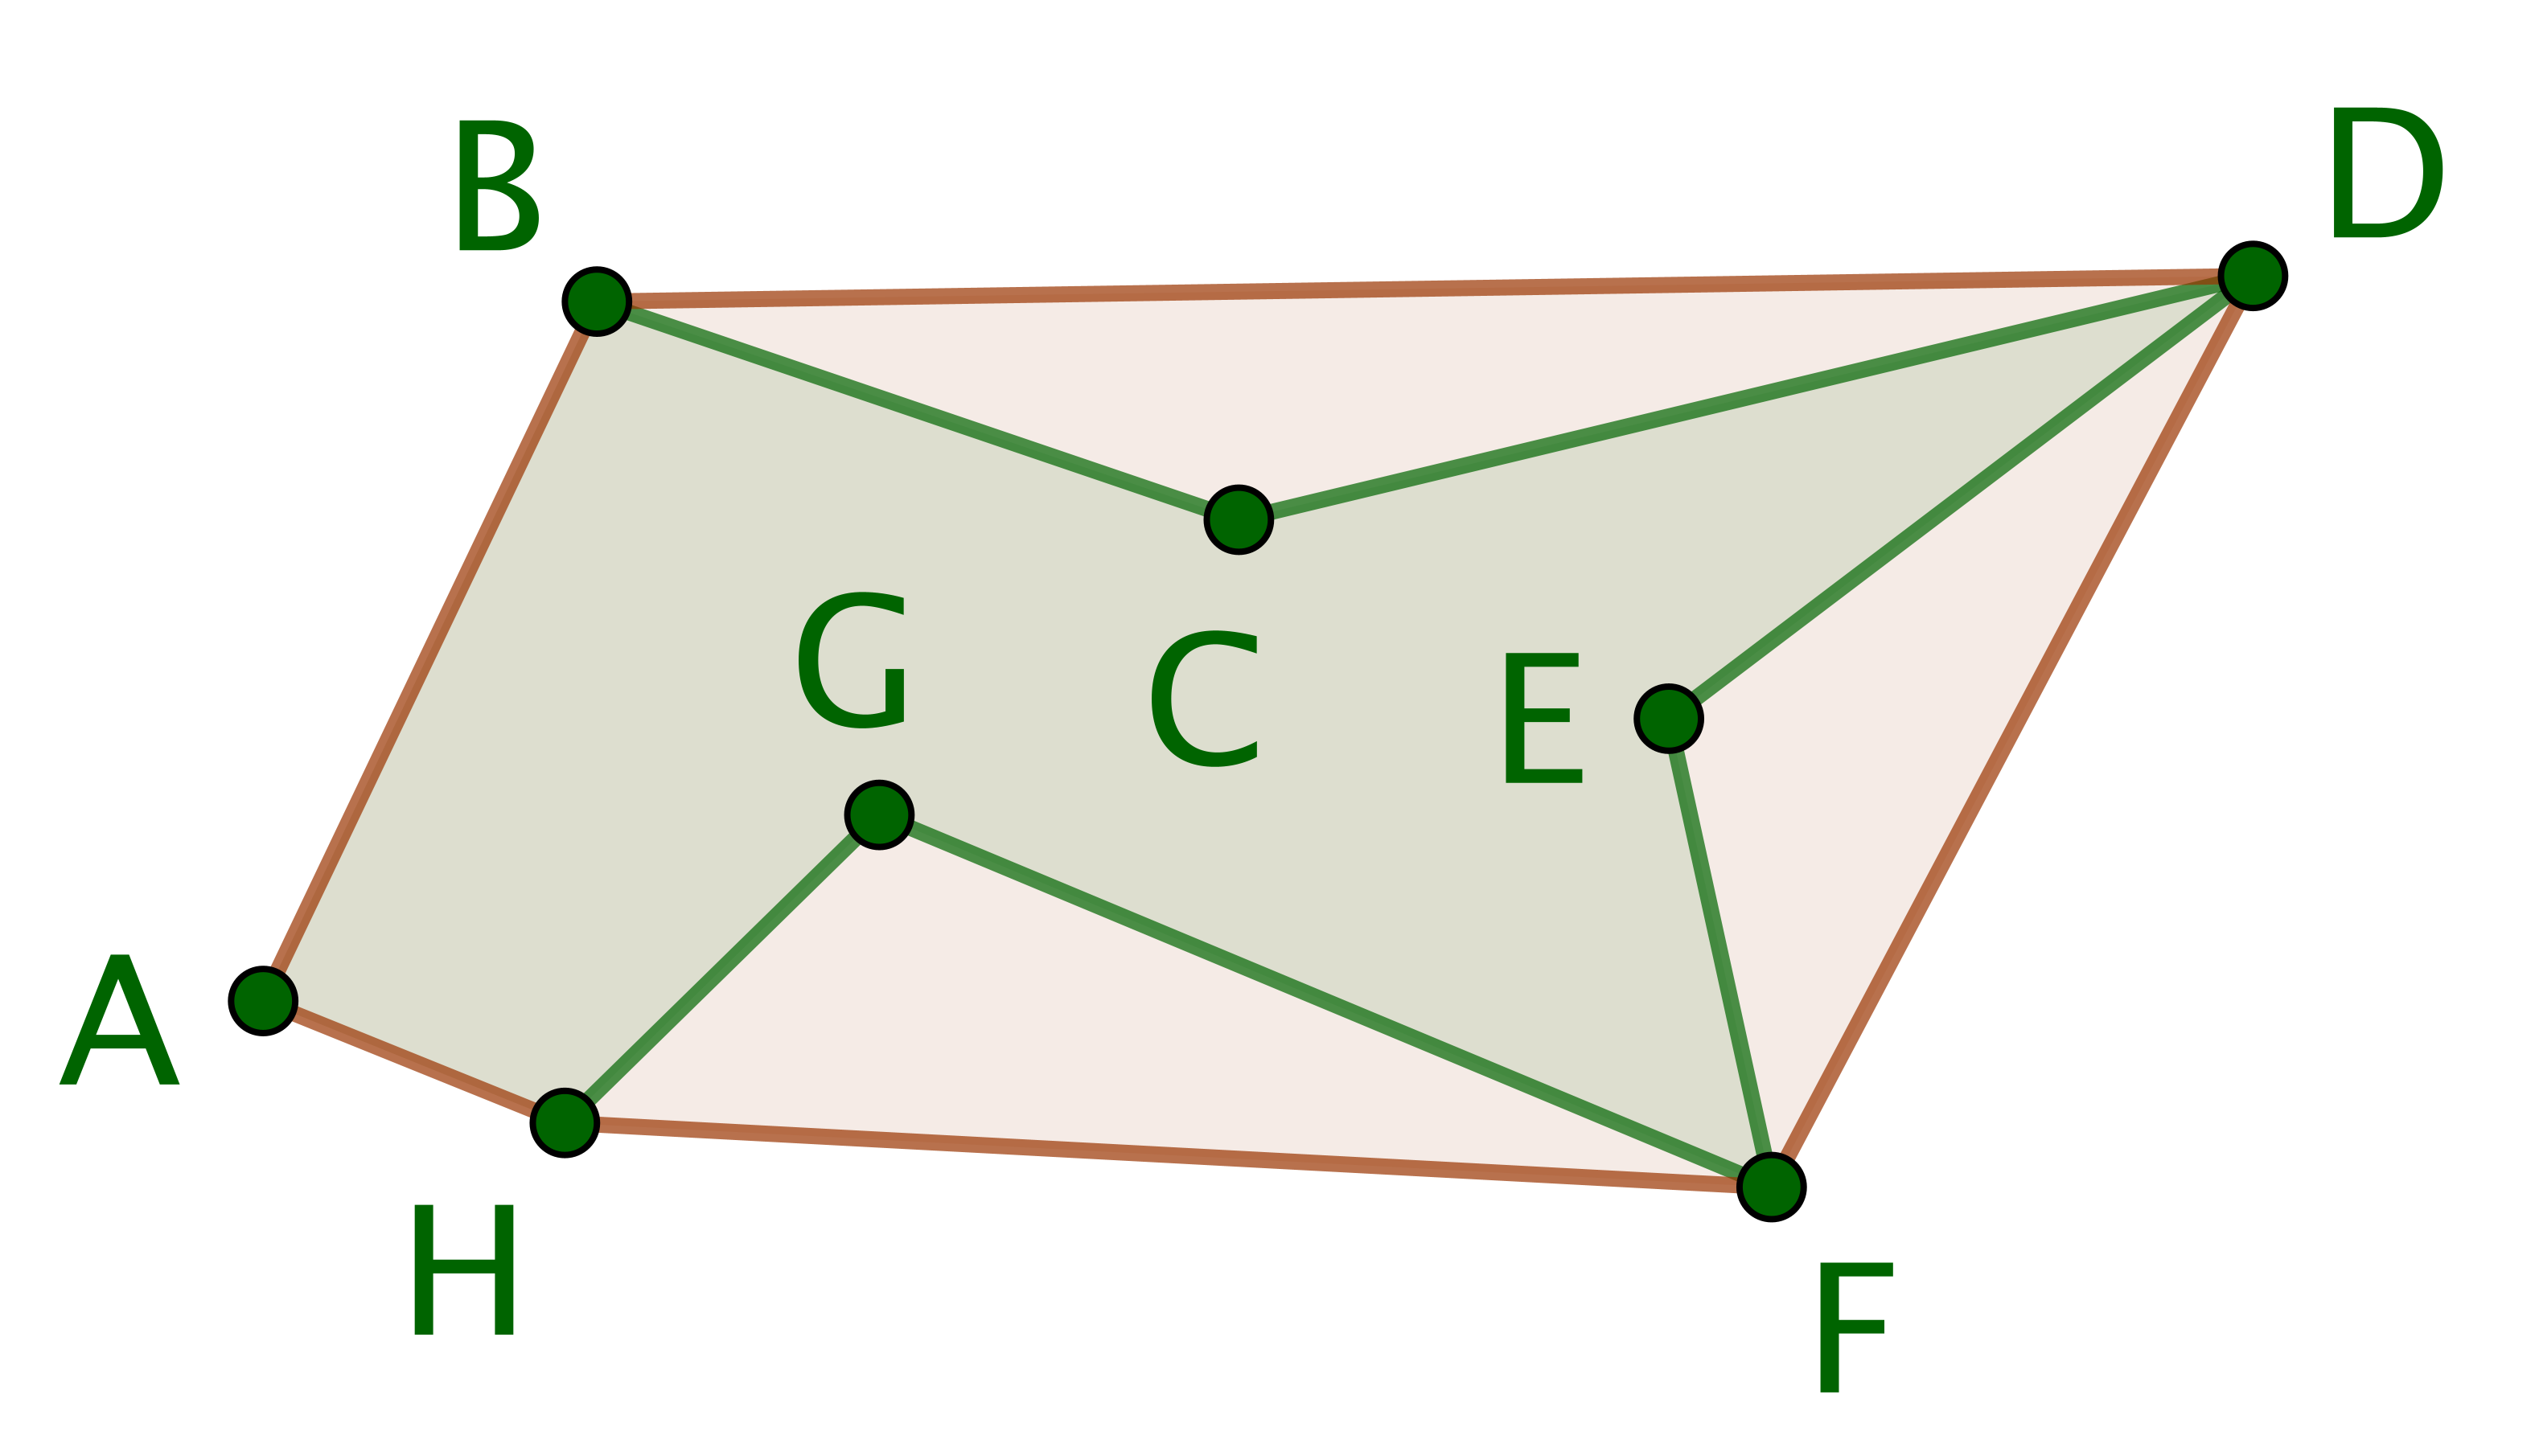
\includegraphics[scale=.45]{content/polygon/sol-must-be/convex-hull.png}
	\end{center}
	
		
	Clairement,
	$\perim{\setproba{E}} < \perim{\setproba{P}}$
	et
	$\area{\setproba{E}} > \area{\setproba{P}}$,
	mais
	$\setproba{E}$ est un \xgone{s} avec $s < n$. 
	%
	Pour gérer ce problème, une idée simple, formalisée après, est d'ajouter des sommets assez prêts des côtés de $\setproba{E}$ pour garder 
	la convexité, 
	un périmètre inférieur à $\perim{\setproba{P}}$, 
	et
	une aire supérieure à $\area{\setproba{P}}$.
	Si c'est faisable, une homothétie de rapport $r \geq 1$, où $r = \frac{ \perim{\setproba{P}} }{ \perim{\setproba{E}} }$, donnera le \ngone\ convexe $\setproba{C}$ cherché.
	La figure suivante illustre cette idée.
	
	\begin{center}
		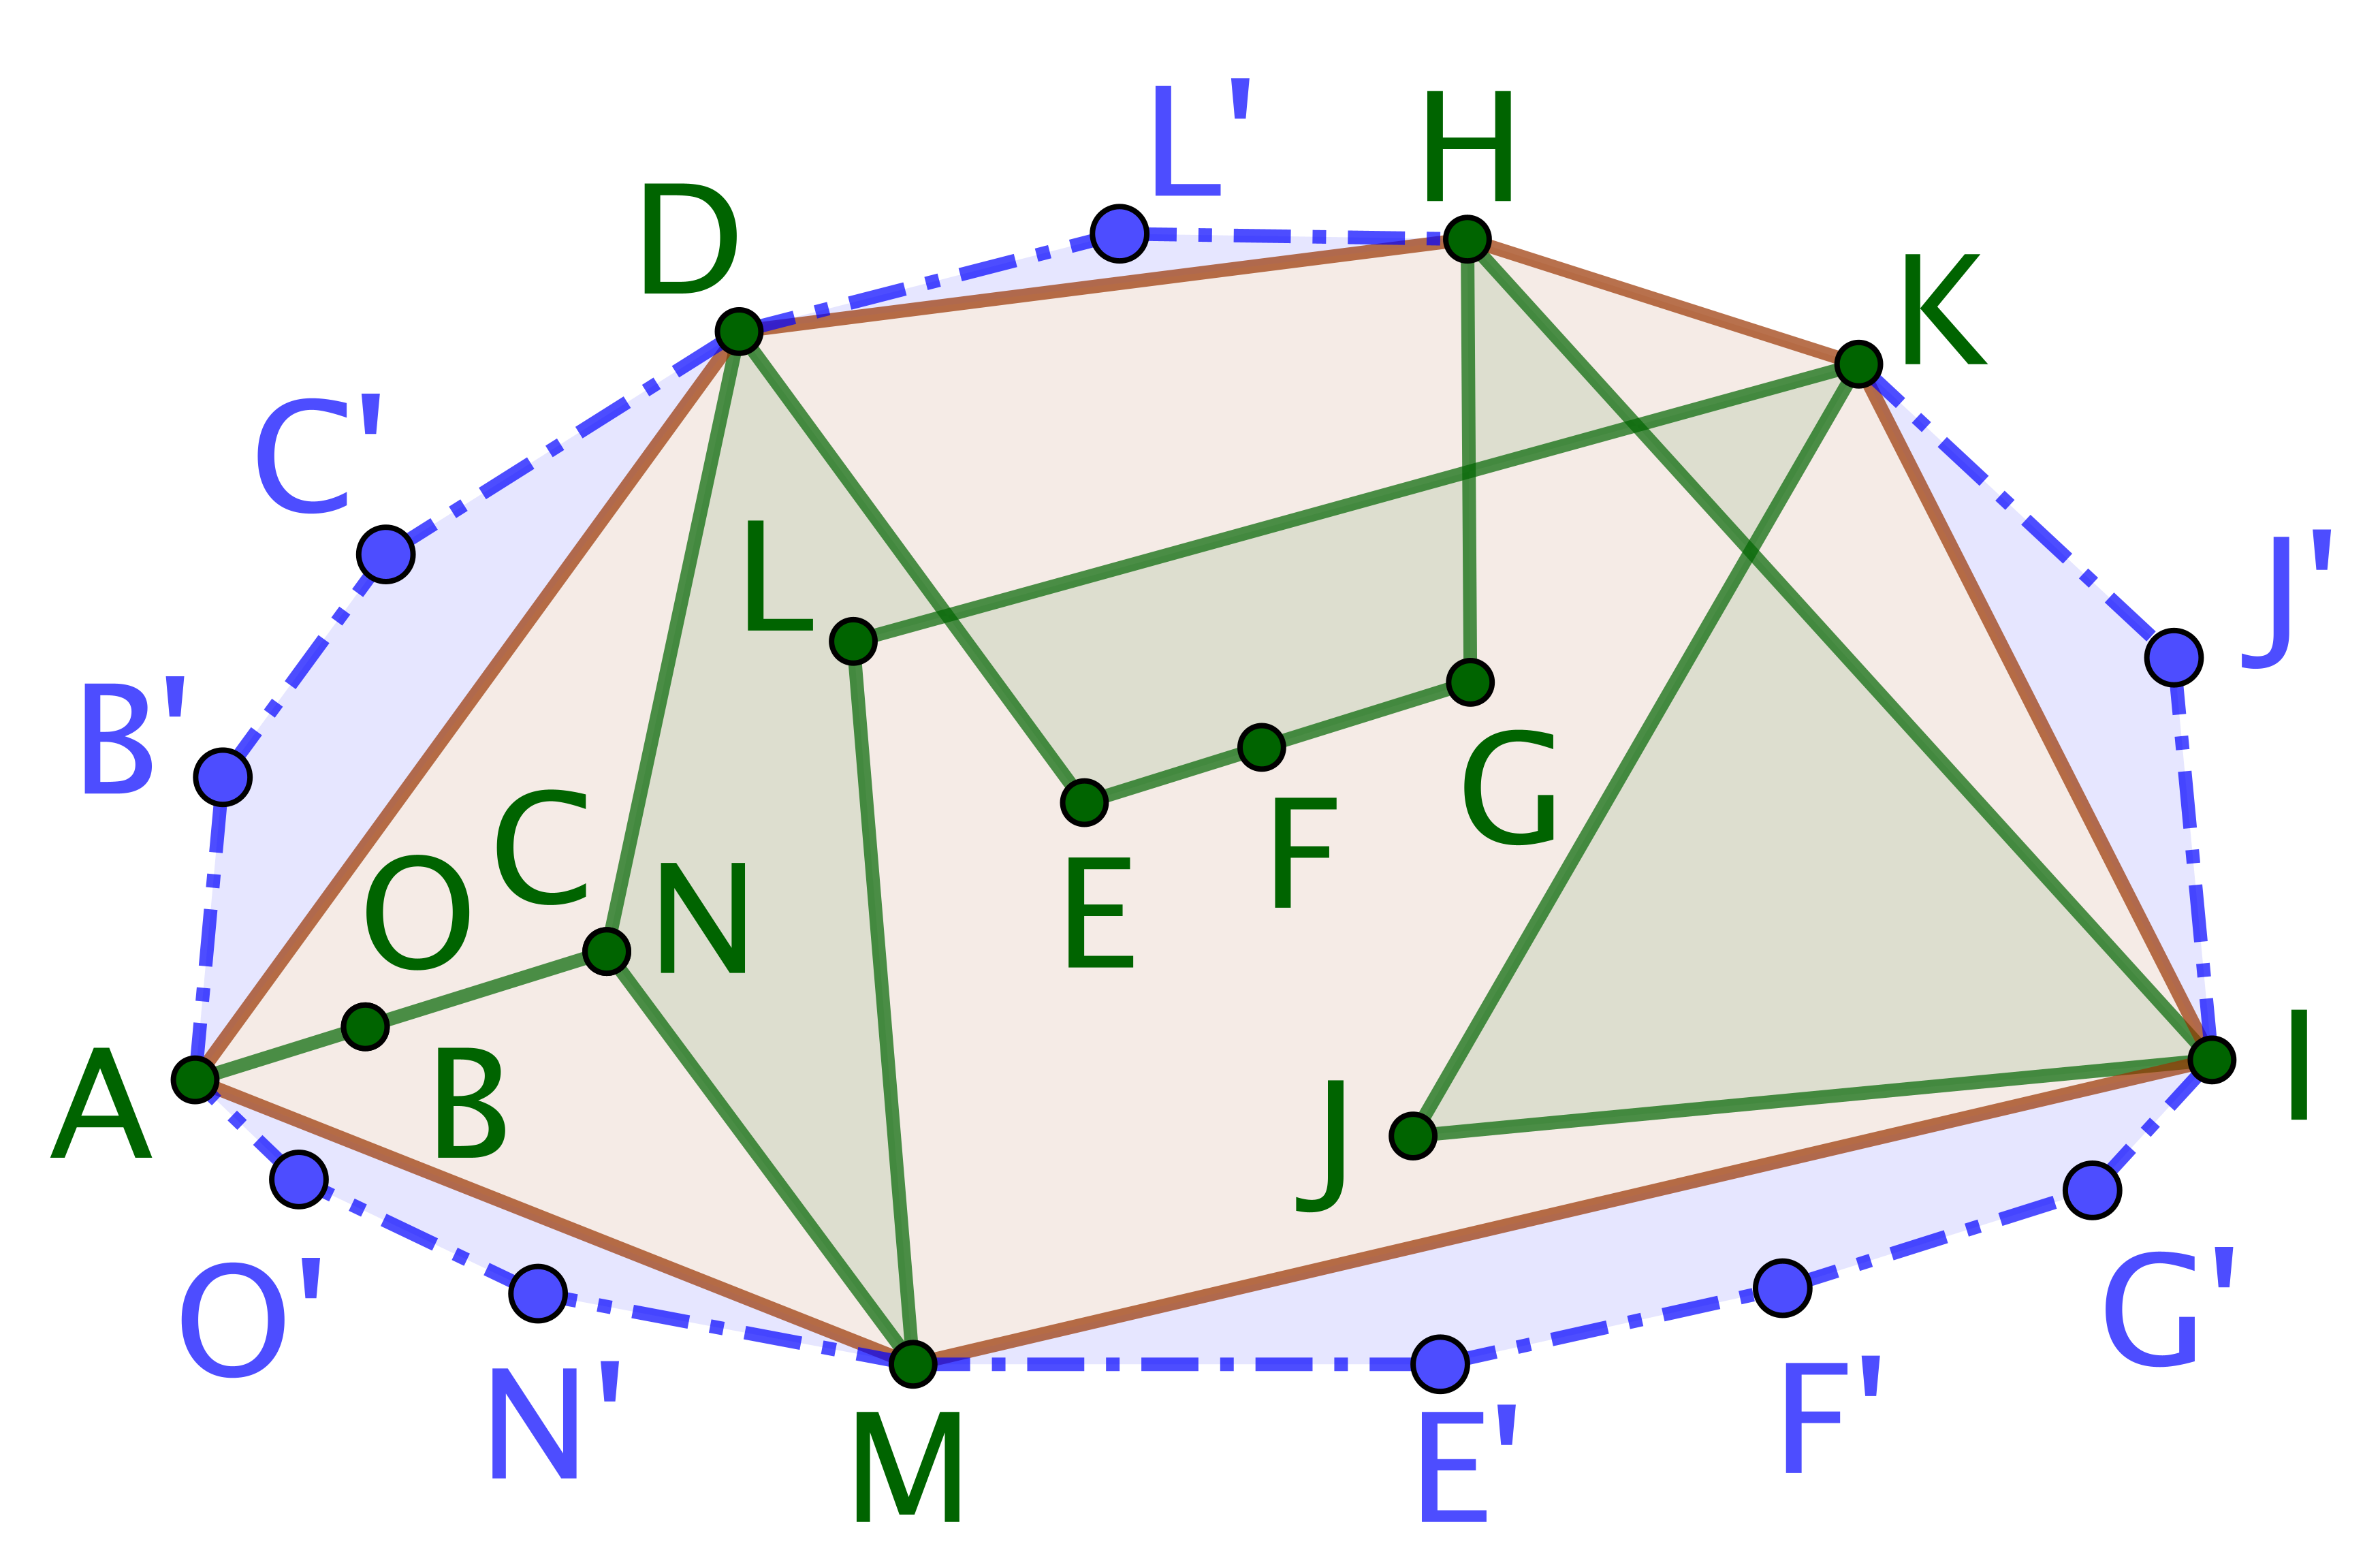
\includegraphics[scale=.45]{content/polygon/sol-must-be/convex-hull-distortion.png}
	\end{center}

	\newpage % TEMPO

	Notons $m = n - s$ qui compte les sommets manquants, puis posons
	$\delta = \frac{\perim{\setproba{P}} - \perim{\setproba{E}}}{m}$.
	%
	\begin{enumerate}
		\item \label{add-vertex-start}
		Considérons $[AB]$ un côté quelconque de $\setproba{E}$.
		Les droites portées par les côtés \focus{autour} de $[AB]$ \focus{dessinent} une région contenant toujours un triangle $ABC$ dont l'intérieur est à l'extérieur
		\footnote{
			C'est ce que l'on appelle de la \focus{low poetry},.
		}
		de $\setproba{E}$ comme dans les deux cas ci-dessous.
		%
		\begin{multicols}{2}
			\centering

			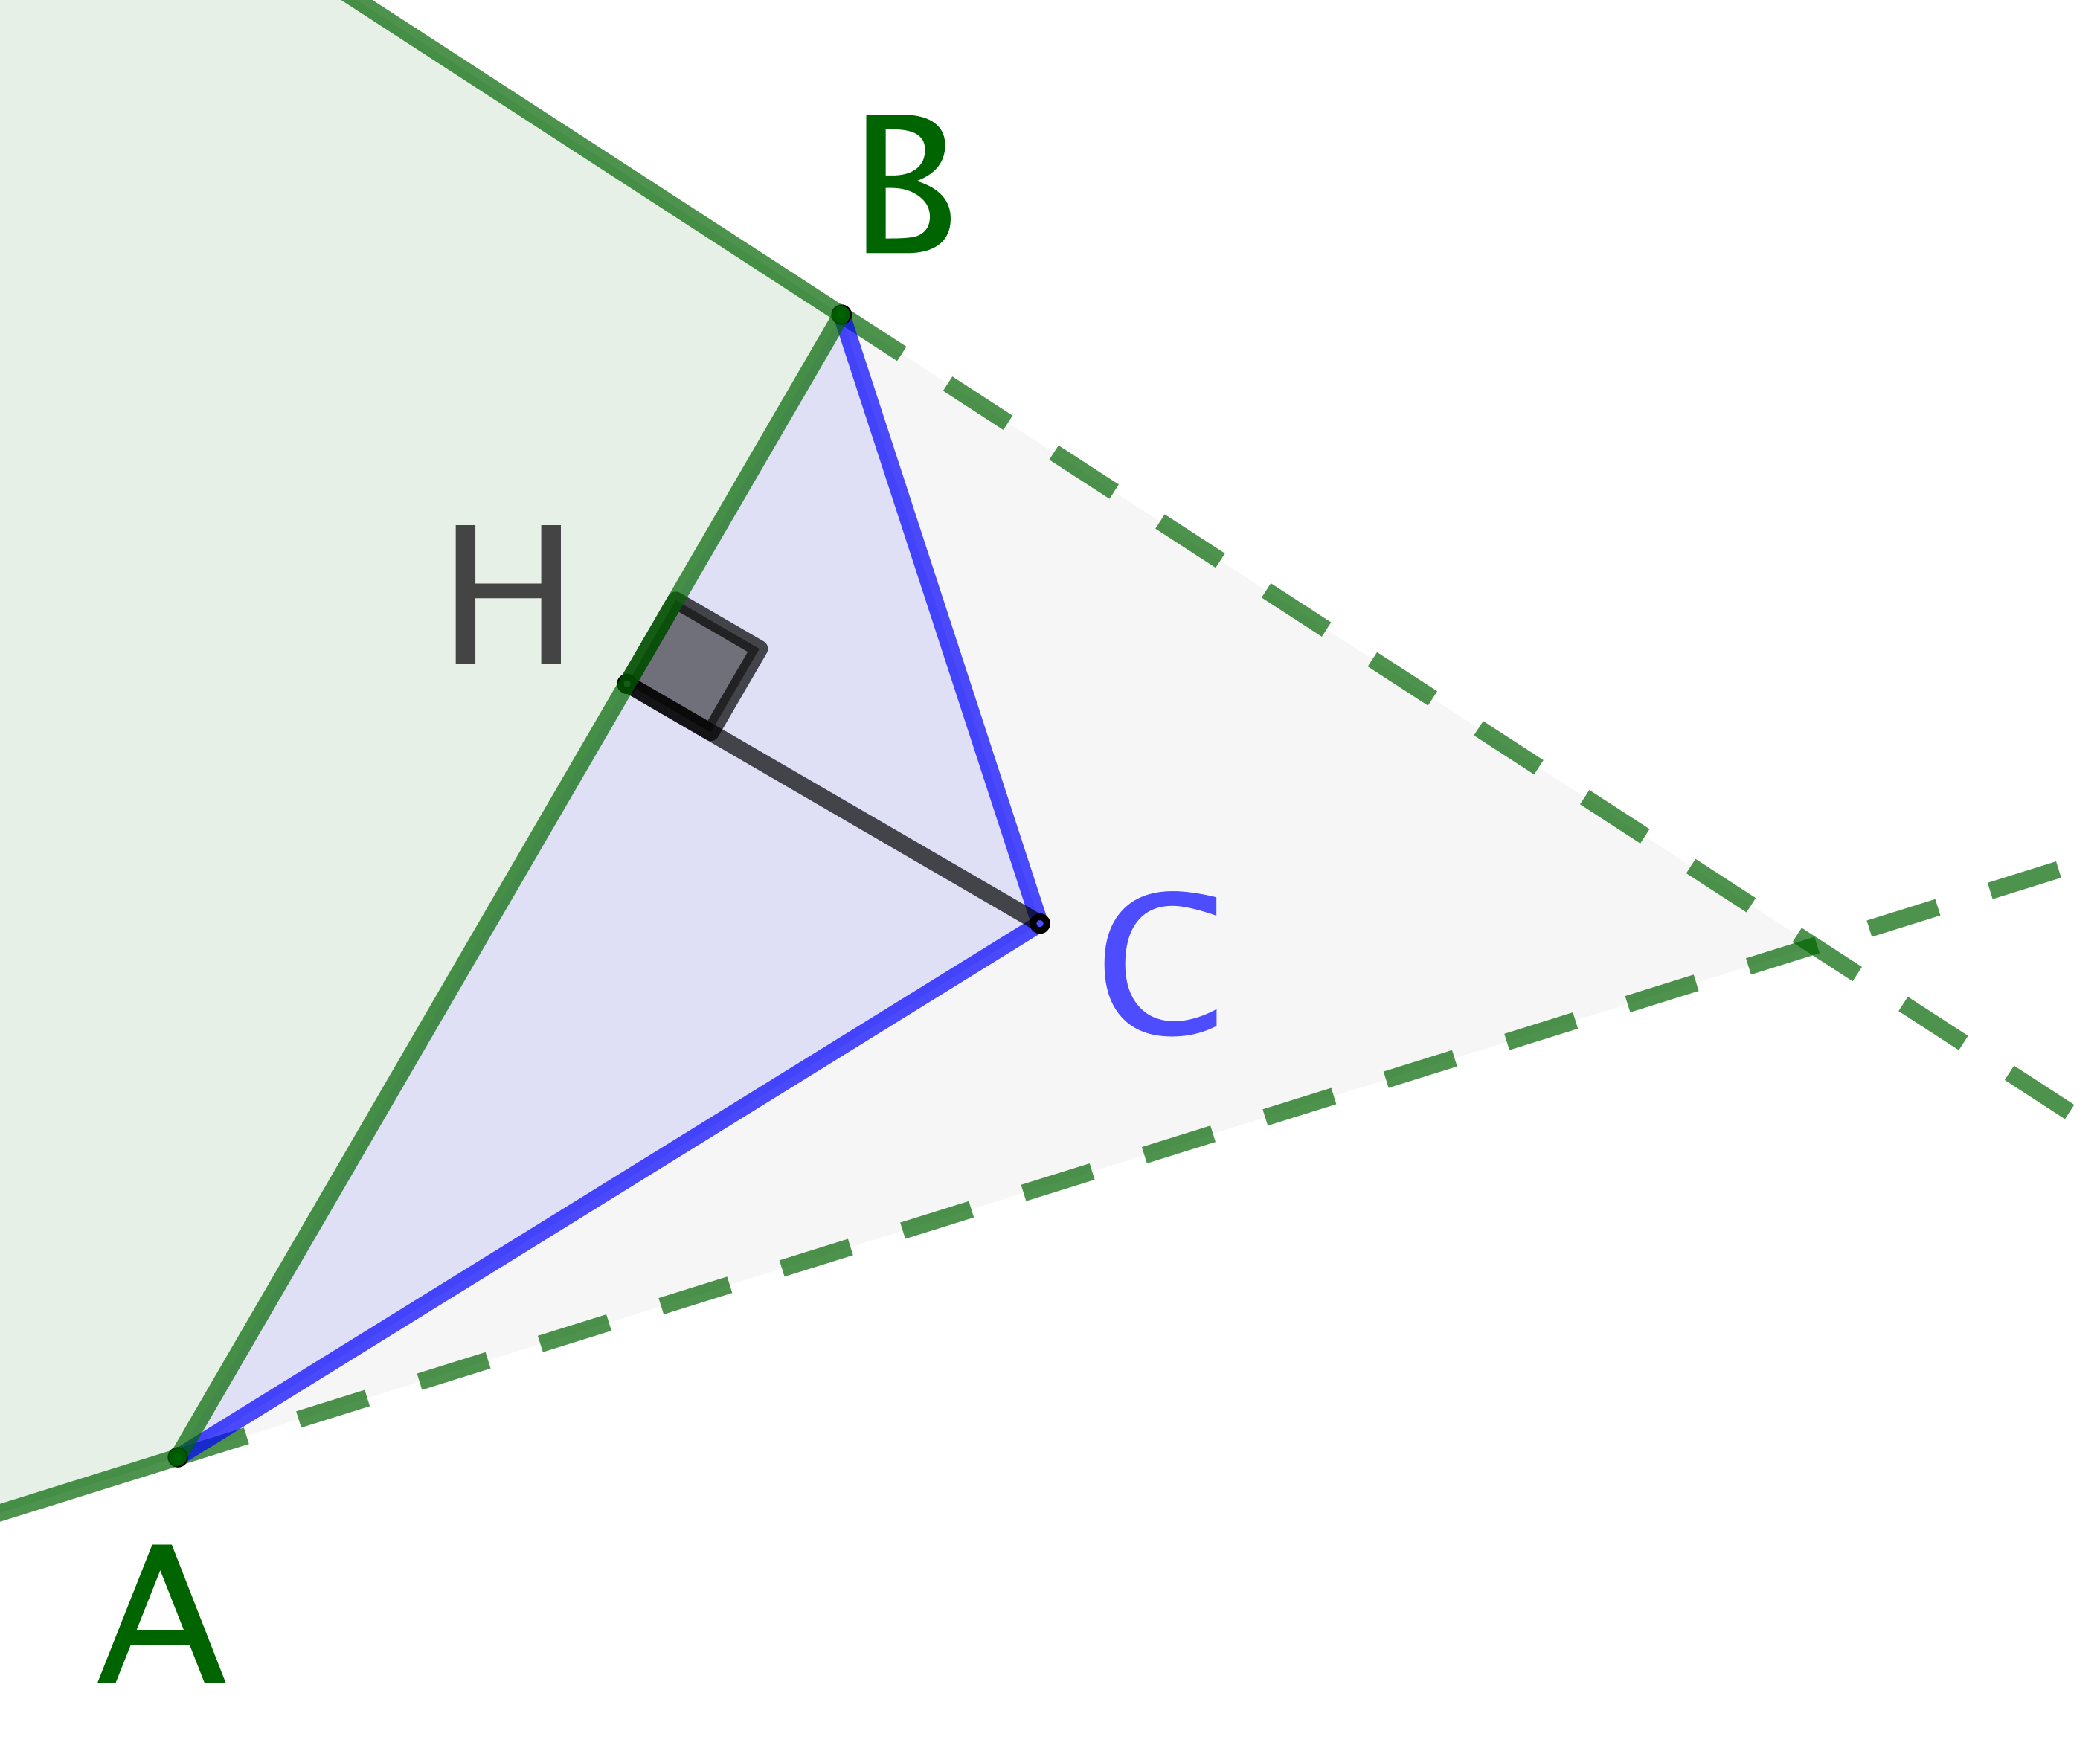
\includegraphics[scale=.35]{content/polygon/sol-must-be/add-vertex-1.png}

			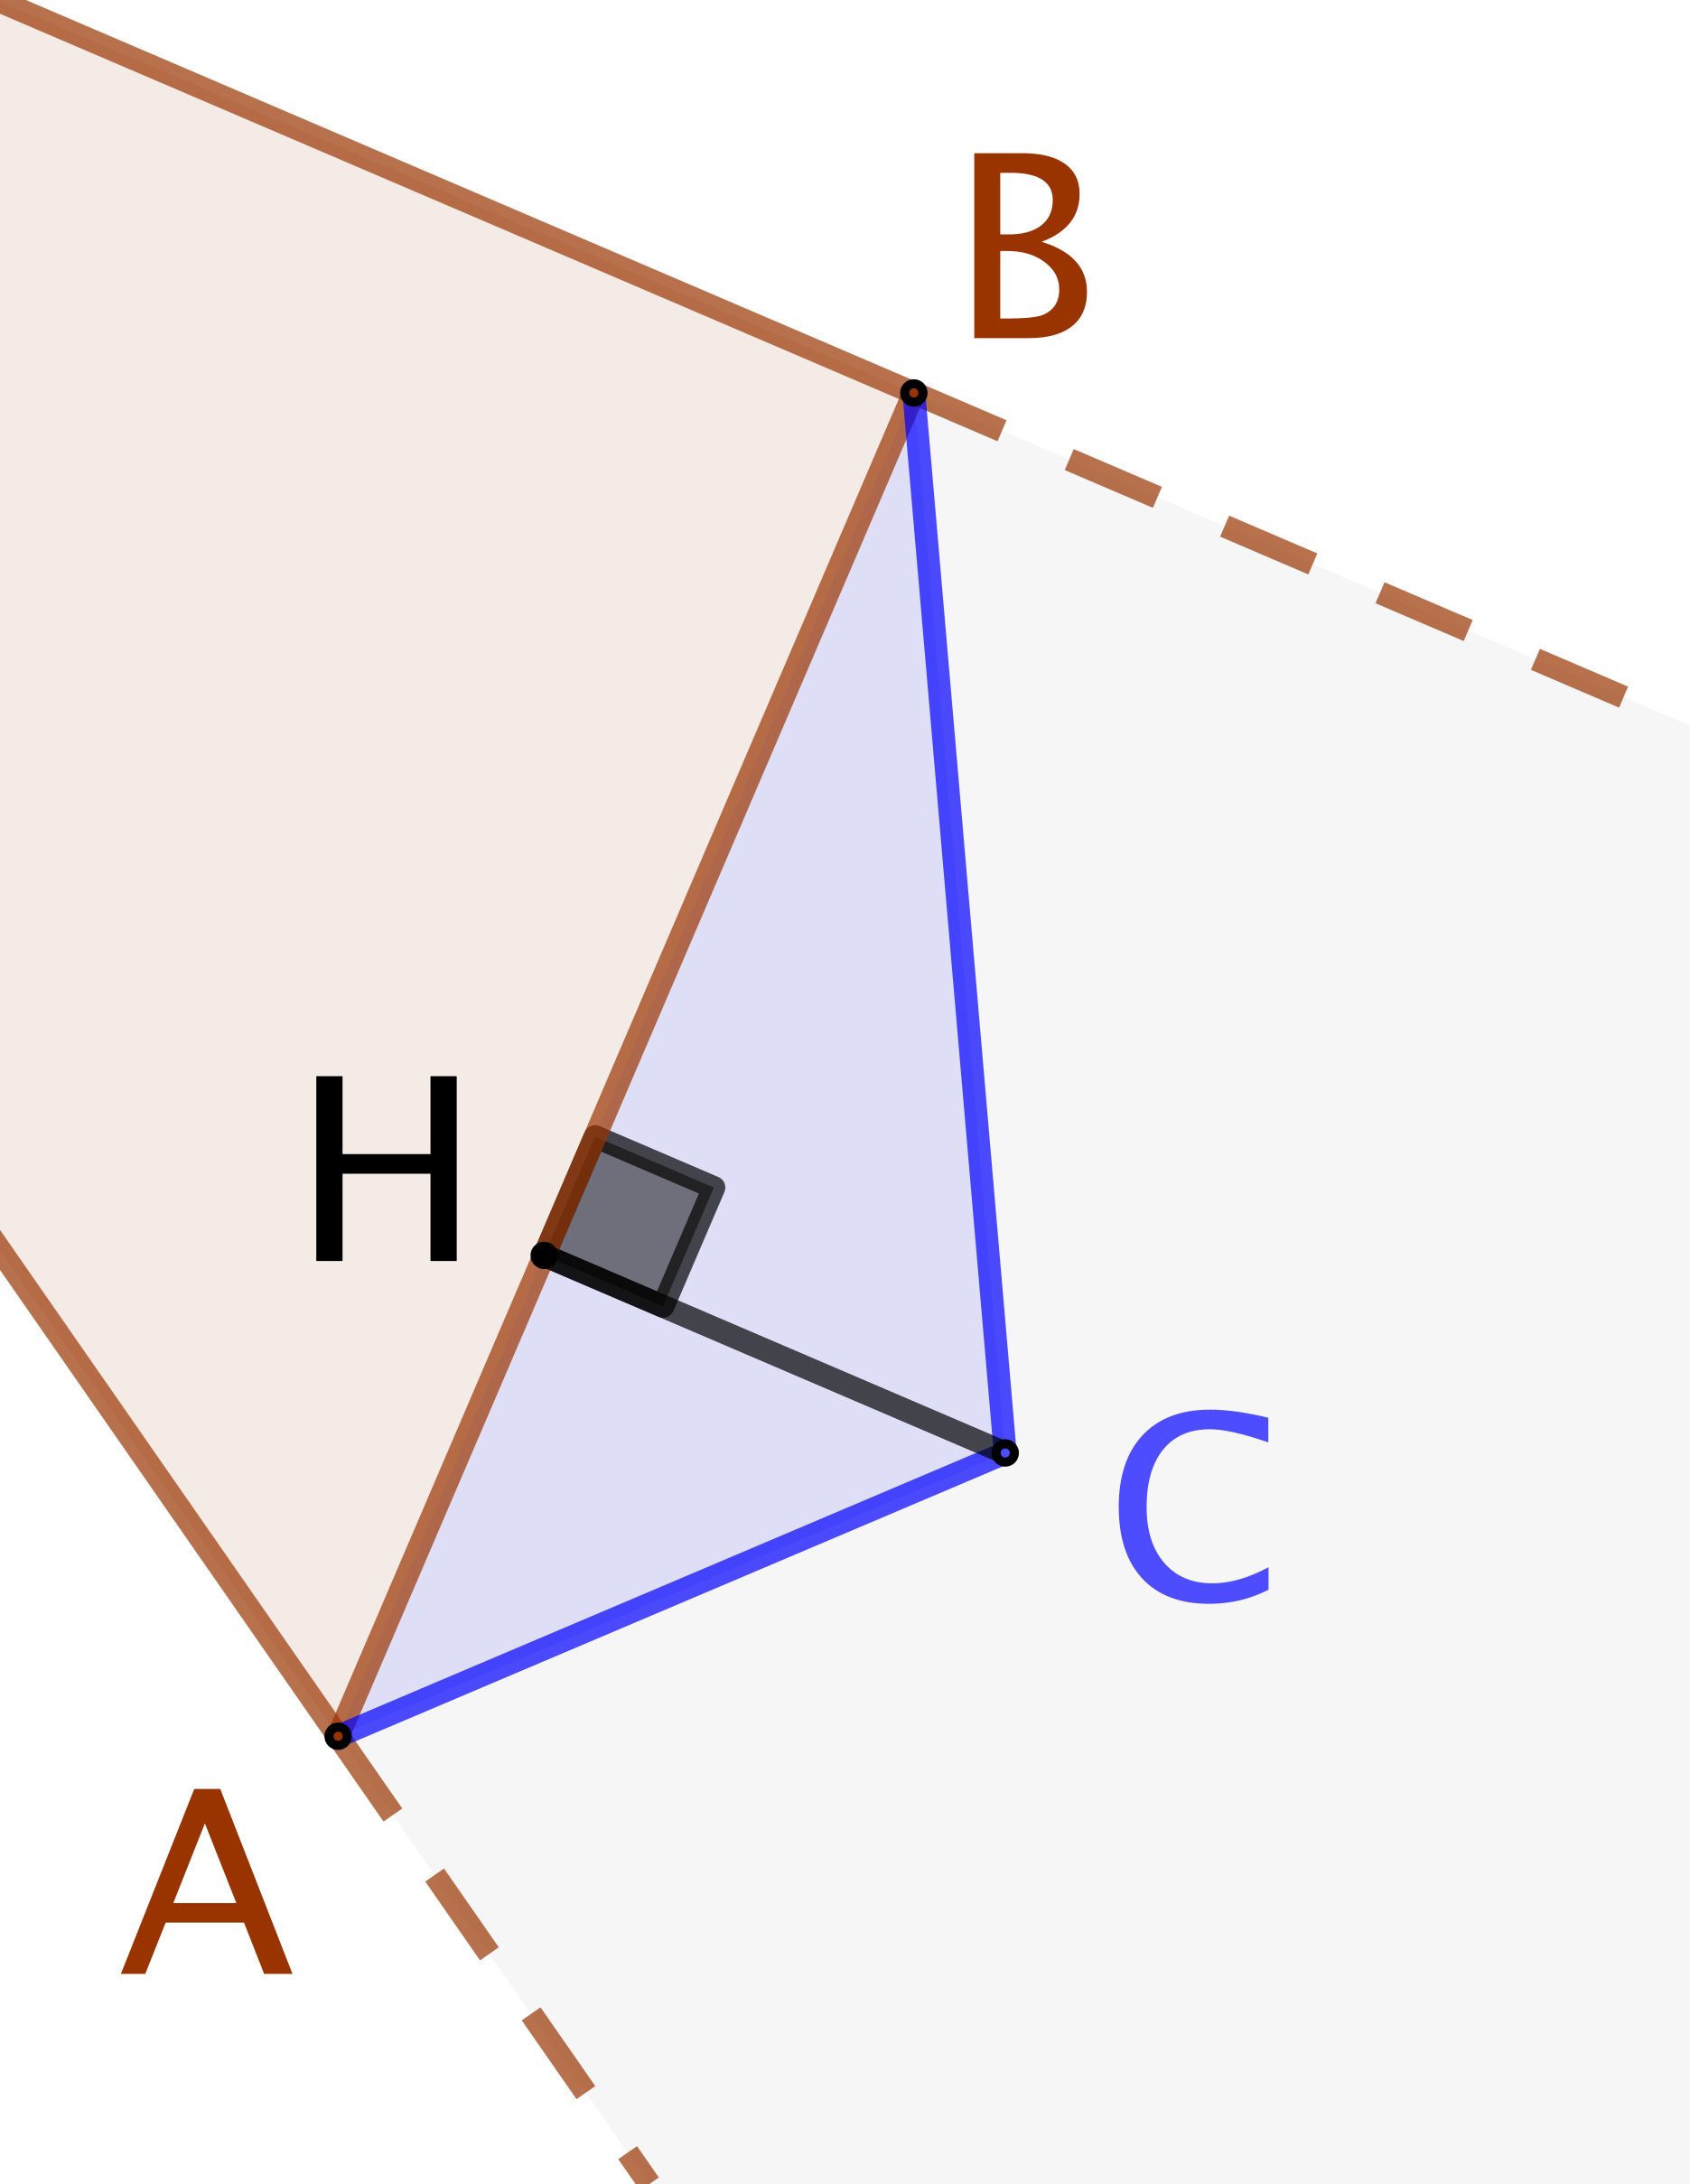
\includegraphics[scale=.35]{content/polygon/sol-must-be/add-vertex-2.png}
		\end{multicols}

		\item Clairement, le polygone $\setproba{E}_+$ obtenu à partir de $\setproba{E}$ en remplaçant le côté $[AB]$ par les côtés $[AC]$ et $[CB]$ est un convexe avec un sommet de plus que $\setproba{E}$.

		\item \label{add-vertex-end}
		Comme $HC$ peut être rendu aussi proche de $0$ que souhaité, il est aisé de voir que l'nous pouvons choisir cette distance de sorte que $AC + BC < AB + \delta$.
		Dès lors, le périmètre de $\setproba{E}_+$ augmente inférieurement strictement à $\delta$ relativement à $\setproba{E}$.

		\item En répétant $(m-1)$ fois les étapes \ref{add-vertex-start} à \ref{add-vertex-end}, nous obtenons un \ngone\ convexe $\setproba{C}$ tel que
		$\area{\setproba{C}} > \area{\setproba{P}}$
		et
		$\perim{\setproba{C}} < \perim{\setproba{E}} + m \delta = \perim{\setproba{P}}$.
	\end{enumerate}
	
	\null\vspace{-6ex}
\end{proof}


% ----------------------- %


\begin{fact} \label{must-be-equi}
	Si un \ngone\ convexe $\setproba{P}$ n'est pas équilatéral,
	alors nous pouvons construire un \ngone\ convexe $\primeit{\setproba{P}}$ tel que
	$\perim{\primeit{\setproba{P}}} = \perim{\setproba{P}}$
	et
	$\area{\primeit{\setproba{P}}} > \area{\setproba{P}}$.
\end{fact}


\begin{proof}
	Considérons un \ngone\ convexe non équilatéral $\setproba{P}$.
	%
	Dans ce cas, $\setproba{P}$ admet un triplet de sommets consécutifs $A$, $B$ et $C$ tels que $AB \neq BC$
	(sinon, on obtiendrait de proche en proche l'équilatéralité).
	La construction vue dans la preuve du fait \ref{tri-one-side-fixed} nous donne la solution: voir les deux dessins ci-après dans lesquels $(AC) \parallel (BB^{\,\prime})$.
	Pour le 2\ieme\ cas, il n'est pas possible d'utiliser le triangle $AB^{\,\prime}C$ isocèle en $B^{\,\prime}$ car $(B^{\,\prime}C)$ porte le côté de $\setproba{P}$ de sommet $C$ juste après $[BC]$, mais ce problème se contourne en considérant un point $B^{\,\prime\prime}$ du segment ouvert $]BB^{\,\prime}[$ (si besoin, se reporter au 2\ieme\ dessin de la preuve du fait \ref{tri-one-side-fixed}).
	%
	\begin{multicols}{2}
		\centering

		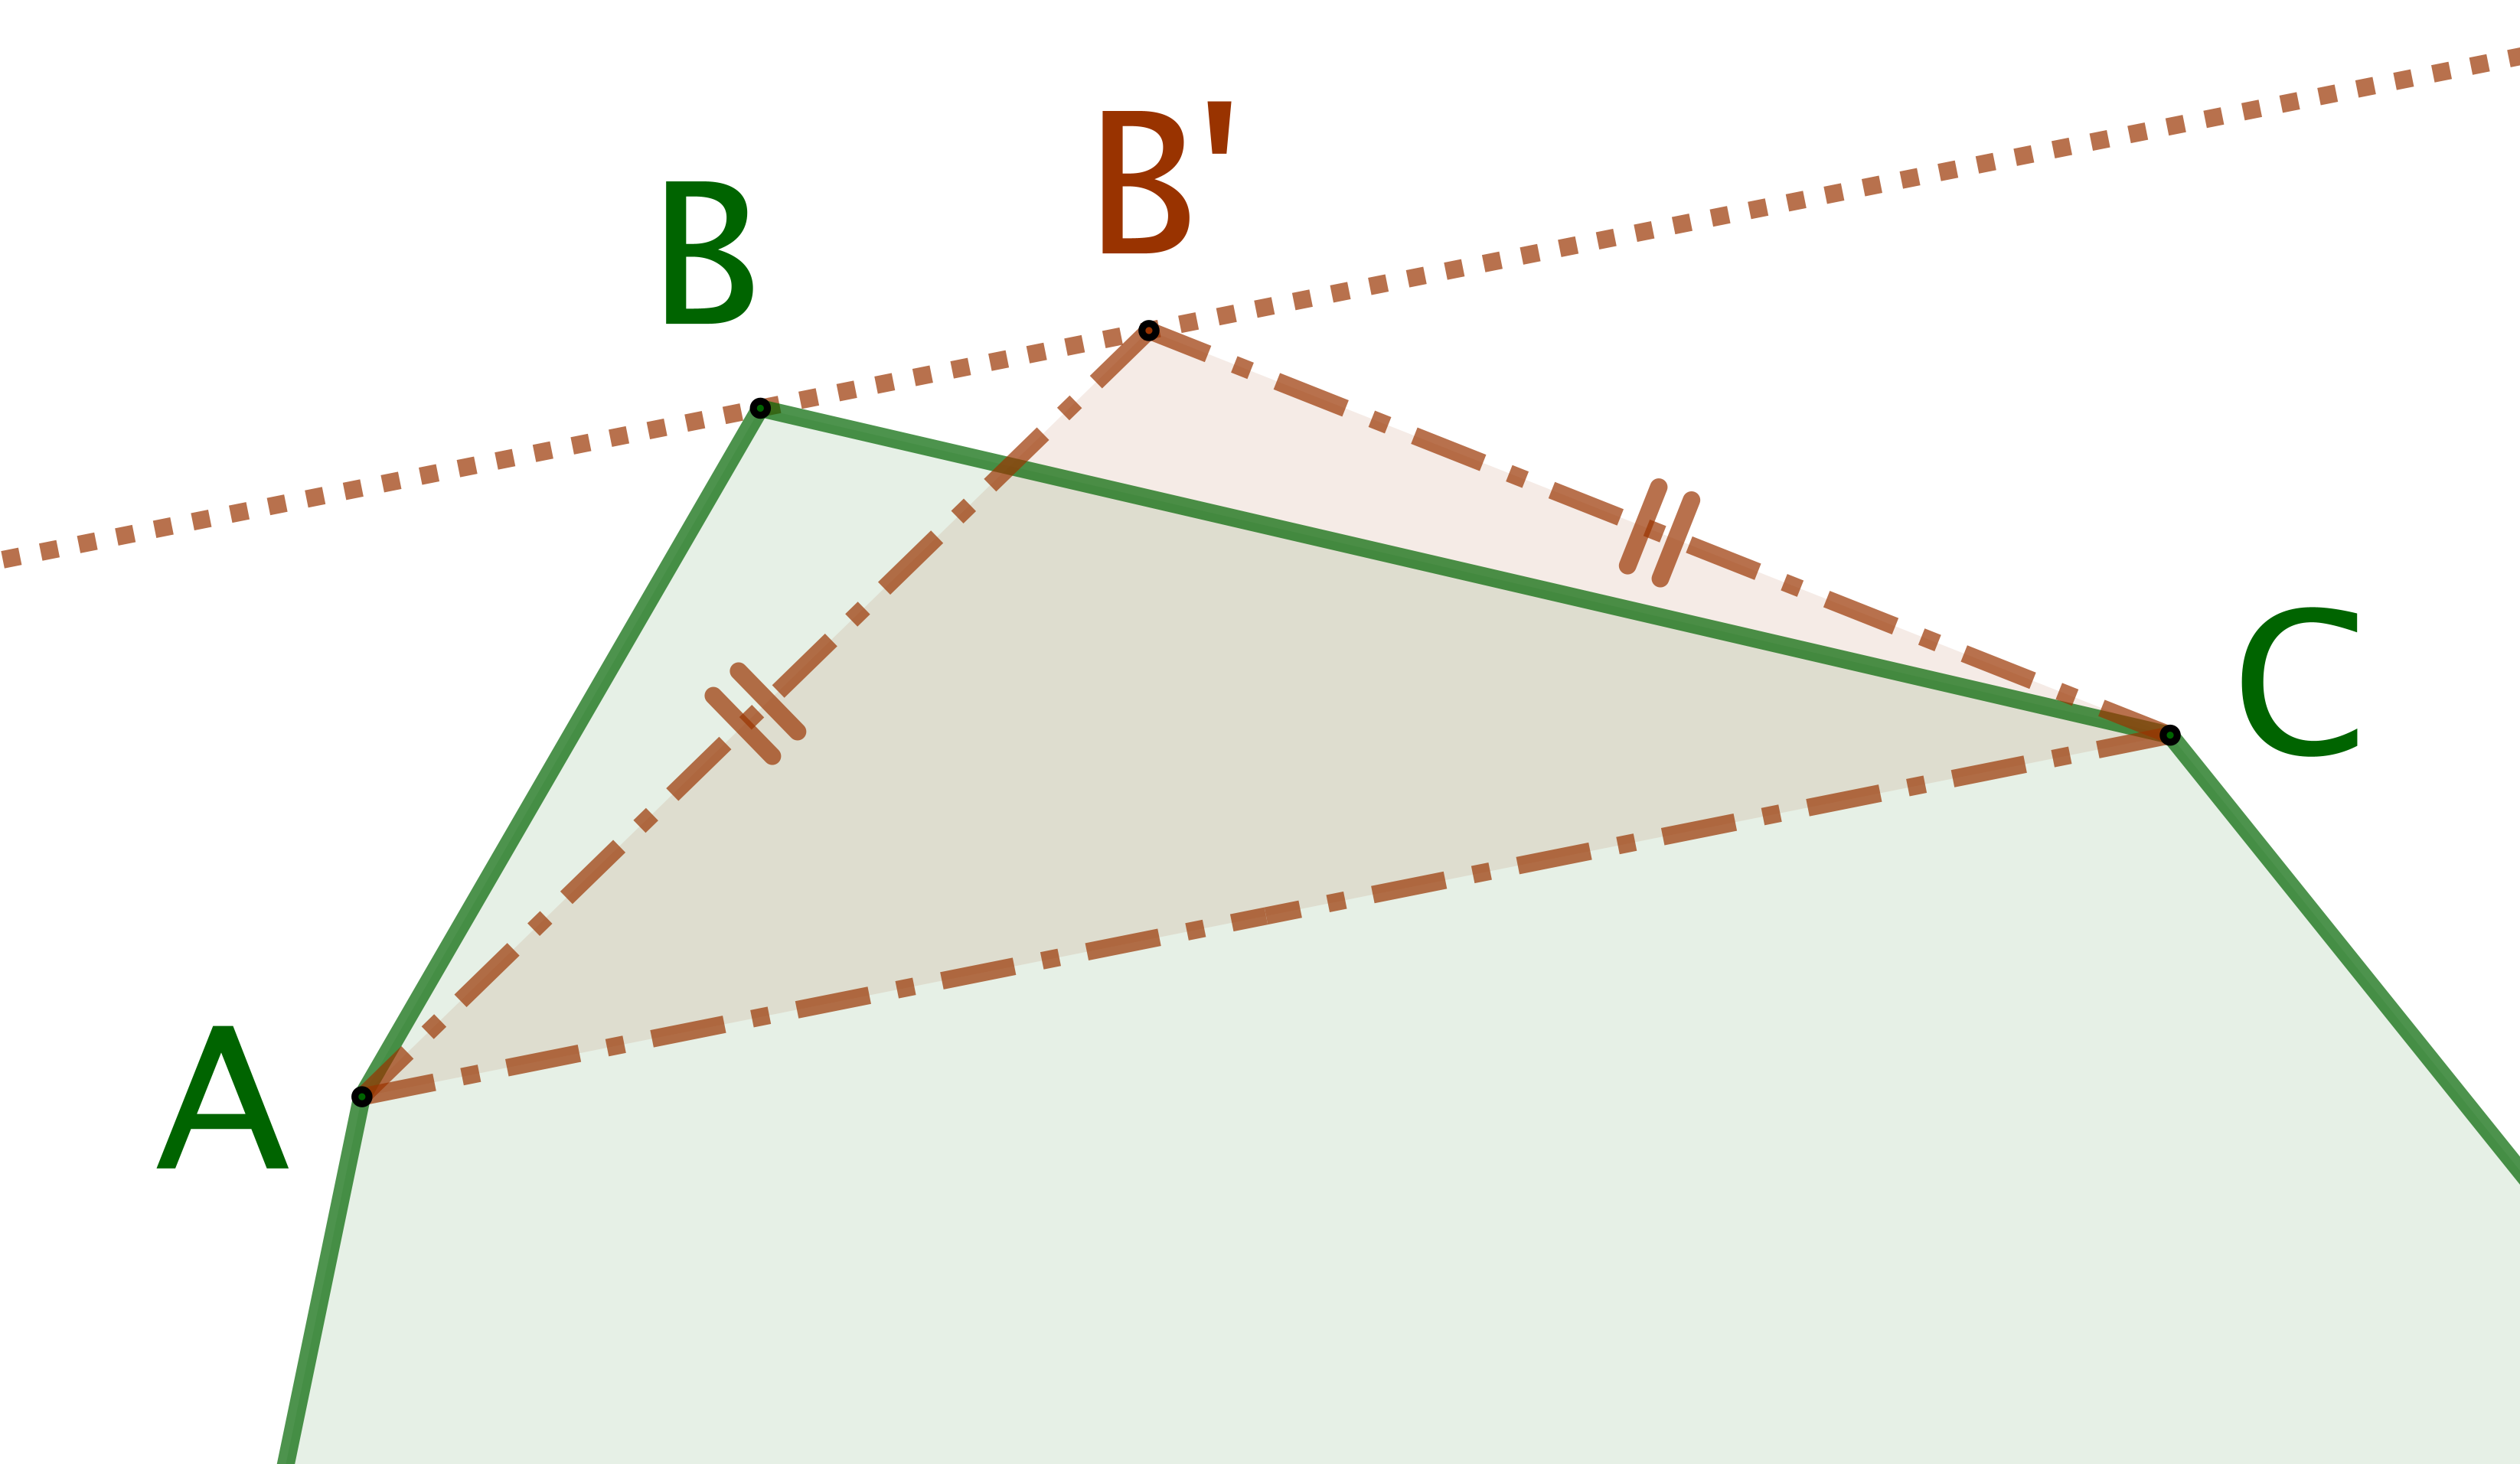
\includegraphics[scale=.4]{content/polygon/sol-must-be/not-iso-OK.png}

		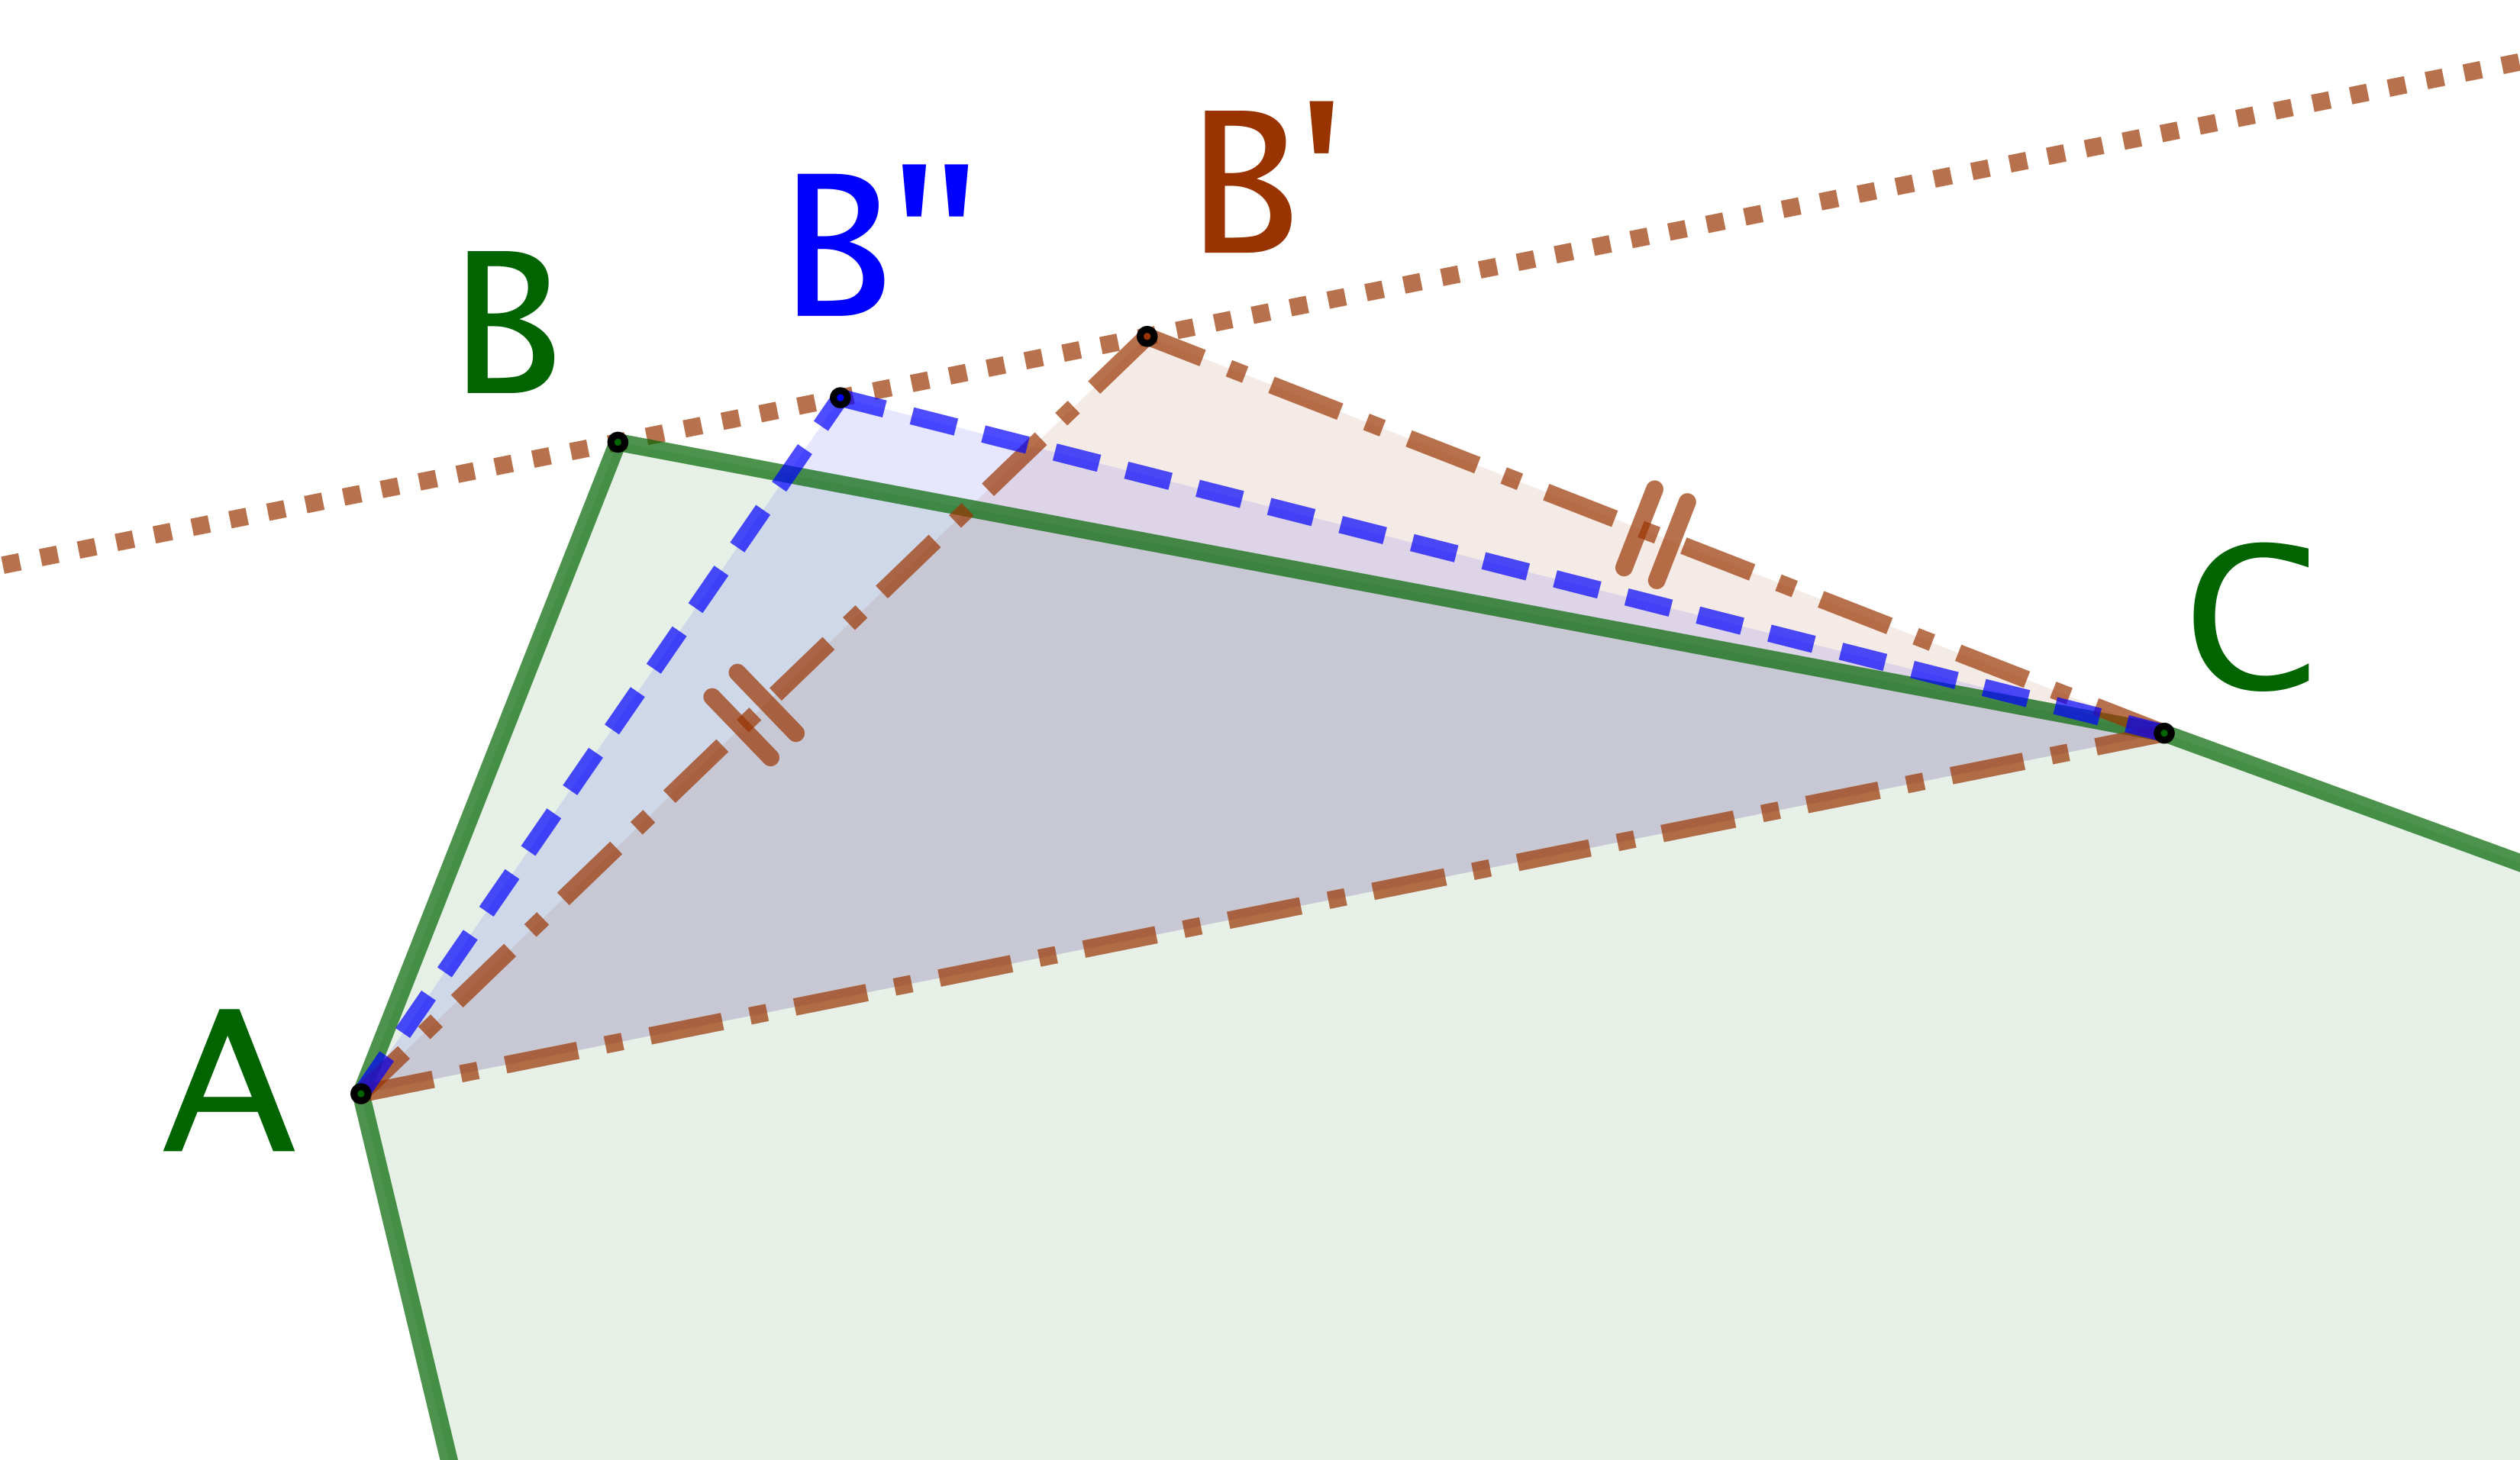
\includegraphics[scale=.4]{content/polygon/sol-must-be/not-iso-KO.png}
	\end{multicols}

	Dans chaque cas, nous avons construit un \ngone\ convexe $\dbleprimeit{\setproba{P}}$ tel que
	$\perim{\dbleprimeit{\setproba{P}}} < \perim{\setproba{P}}$
	et
	$\area{\dbleprimeit{\setproba{P}}} = \area{\setproba{P}}$.
	Une homothétie de rapport $r > 1$, où $r = \frac{ \perim{\setproba{P}} }{ \perim{\setproba{E}} }$, donne un \ngone\ convexe $\primeit{\setproba{P}}$ vérifiant
	$\perim{\primeit{\setproba{P}}} = \perim{\setproba{P}}$
	et
	$\area{\primeit{\setproba{P}}} > \area{\setproba{P}}$.
\end{proof}


\begin{remark}
	Le fait précédent ne permet pas de toujours se ramener au cas d'un \nequi\ convexe. Il nous dit juste que si un \ngone\ convexe maximise son aire à périmètre fixé, alors il devra être, a minima, un \nequi. La nuance est importante, et une similaire existe pour la conclusion du fait suivant.
\end{remark}


% ----------------------- %


\begin{fact} \label{must-be-iso}
	Si un \nequi\ convexe $\setproba{P}$ n'est pas équiangle,
	alors il existe un \ngone\ convexe $\primeit{\setproba{P}}$ tel que
	$\perim{\primeit{\setproba{P}}} = \perim{\setproba{P}}$
	et
	$\area{\primeit{\setproba{P}}} > \area{\setproba{P}}$.
\end{fact}


\begin{proof}
	Considérons un \nequi\ convexe non équiangle $\setproba{P}$.
	%
	Dans ce cas, $\setproba{P}$ admet un quadruplet de sommets consécutifs $A$, $B$, $C$ et $D$ tels que $\anglein{ABC} \neq \anglein{BCD}$
	(sinon, on obtiendrait de proche en proche l'équiangularité).
	Quitte à changer l'ordre de parcours des sommets de $\setproba{P}$, nous pouvons supposer $\anglein{ABC} > \anglein{BCD}$.
	%
	\begin{center}
		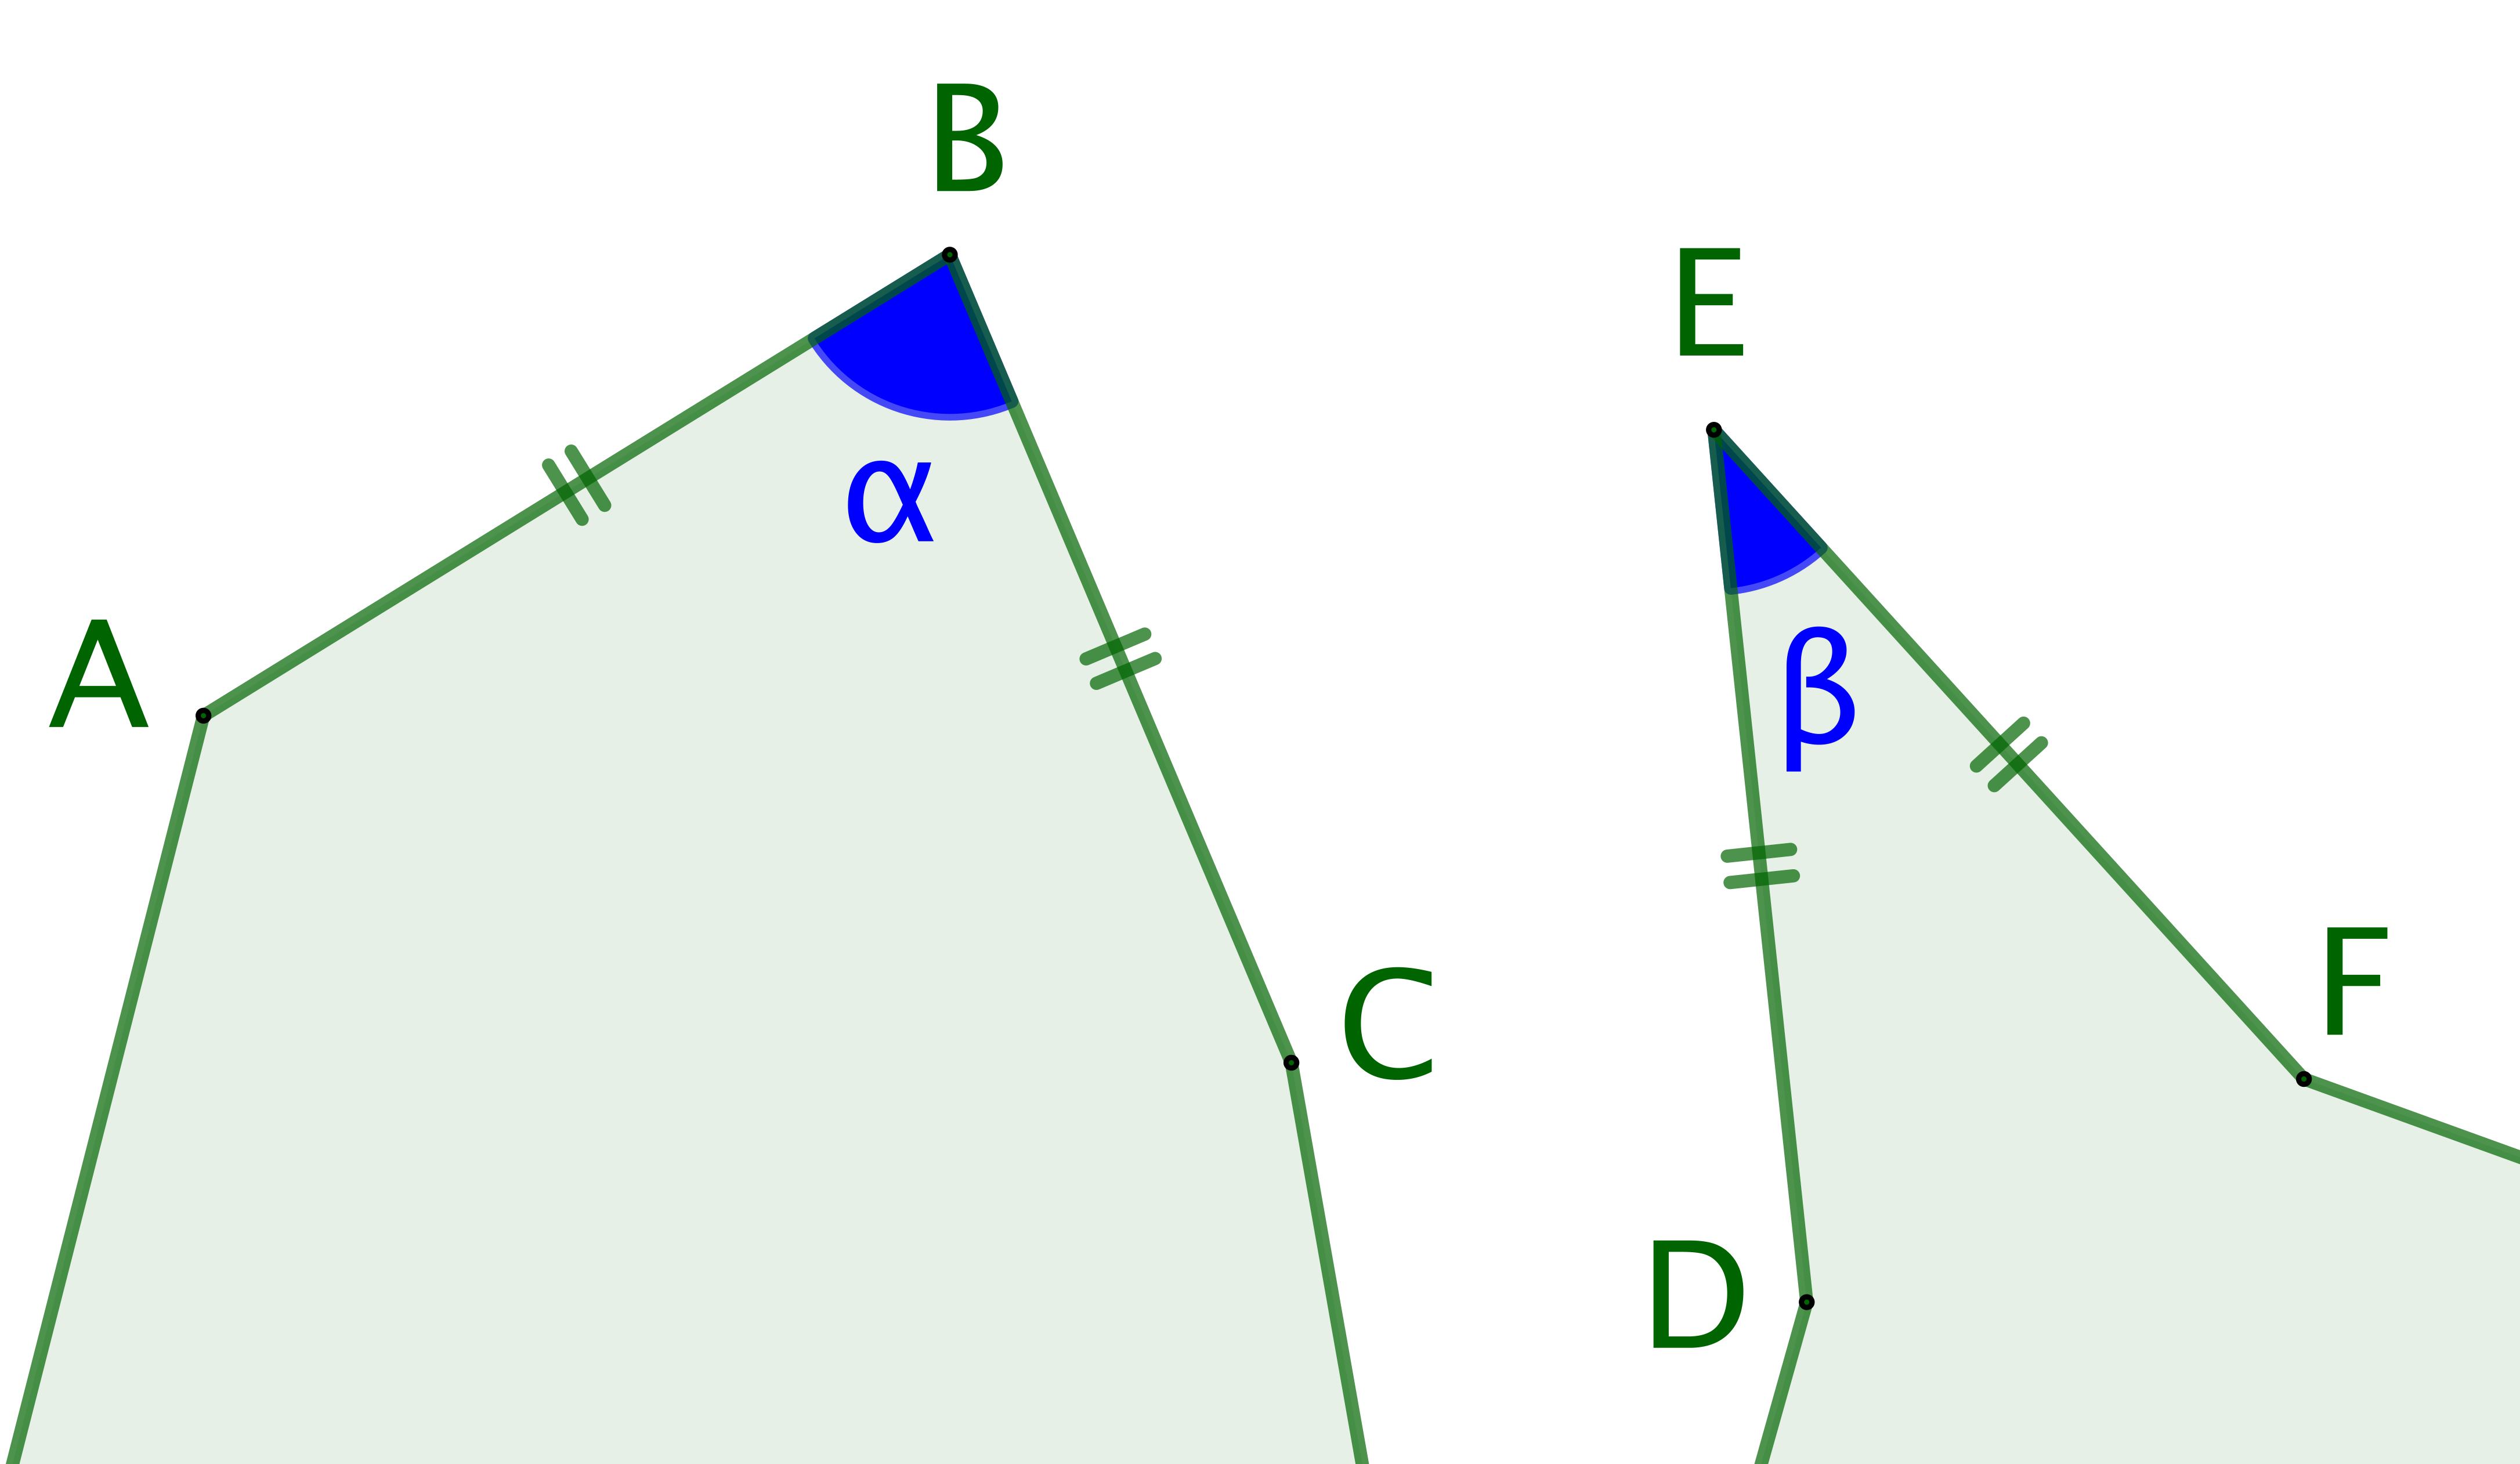
\includegraphics[scale=.4]{content/polygon/sol-must-be/2-eq-angles-start.png}
	\end{center}
	
	En déplaçant $B$ et $C$ dans la zone grise hachurée strictement entre les droites vertes en pointillés, nous garderons un \ngone\ convexe.
	%
	Concentrons-nous donc sur le quadrilatère $ABCD$, et posons $c = AB$ la longueur commune des côtés de $\setproba{P}$, ainsi que $d = AD$ que nous ne pouvons pas modifier.
	%
	Si nous fixons la valeur de $c$, notre situation possède juste un degré de liberté comme le montre la construction de $C$ ci-après qui utilise des cercles de rayon $c$ centrés en $A$ et $D$ fixes, et $B$ mobile.
	%
	\begin{center}
		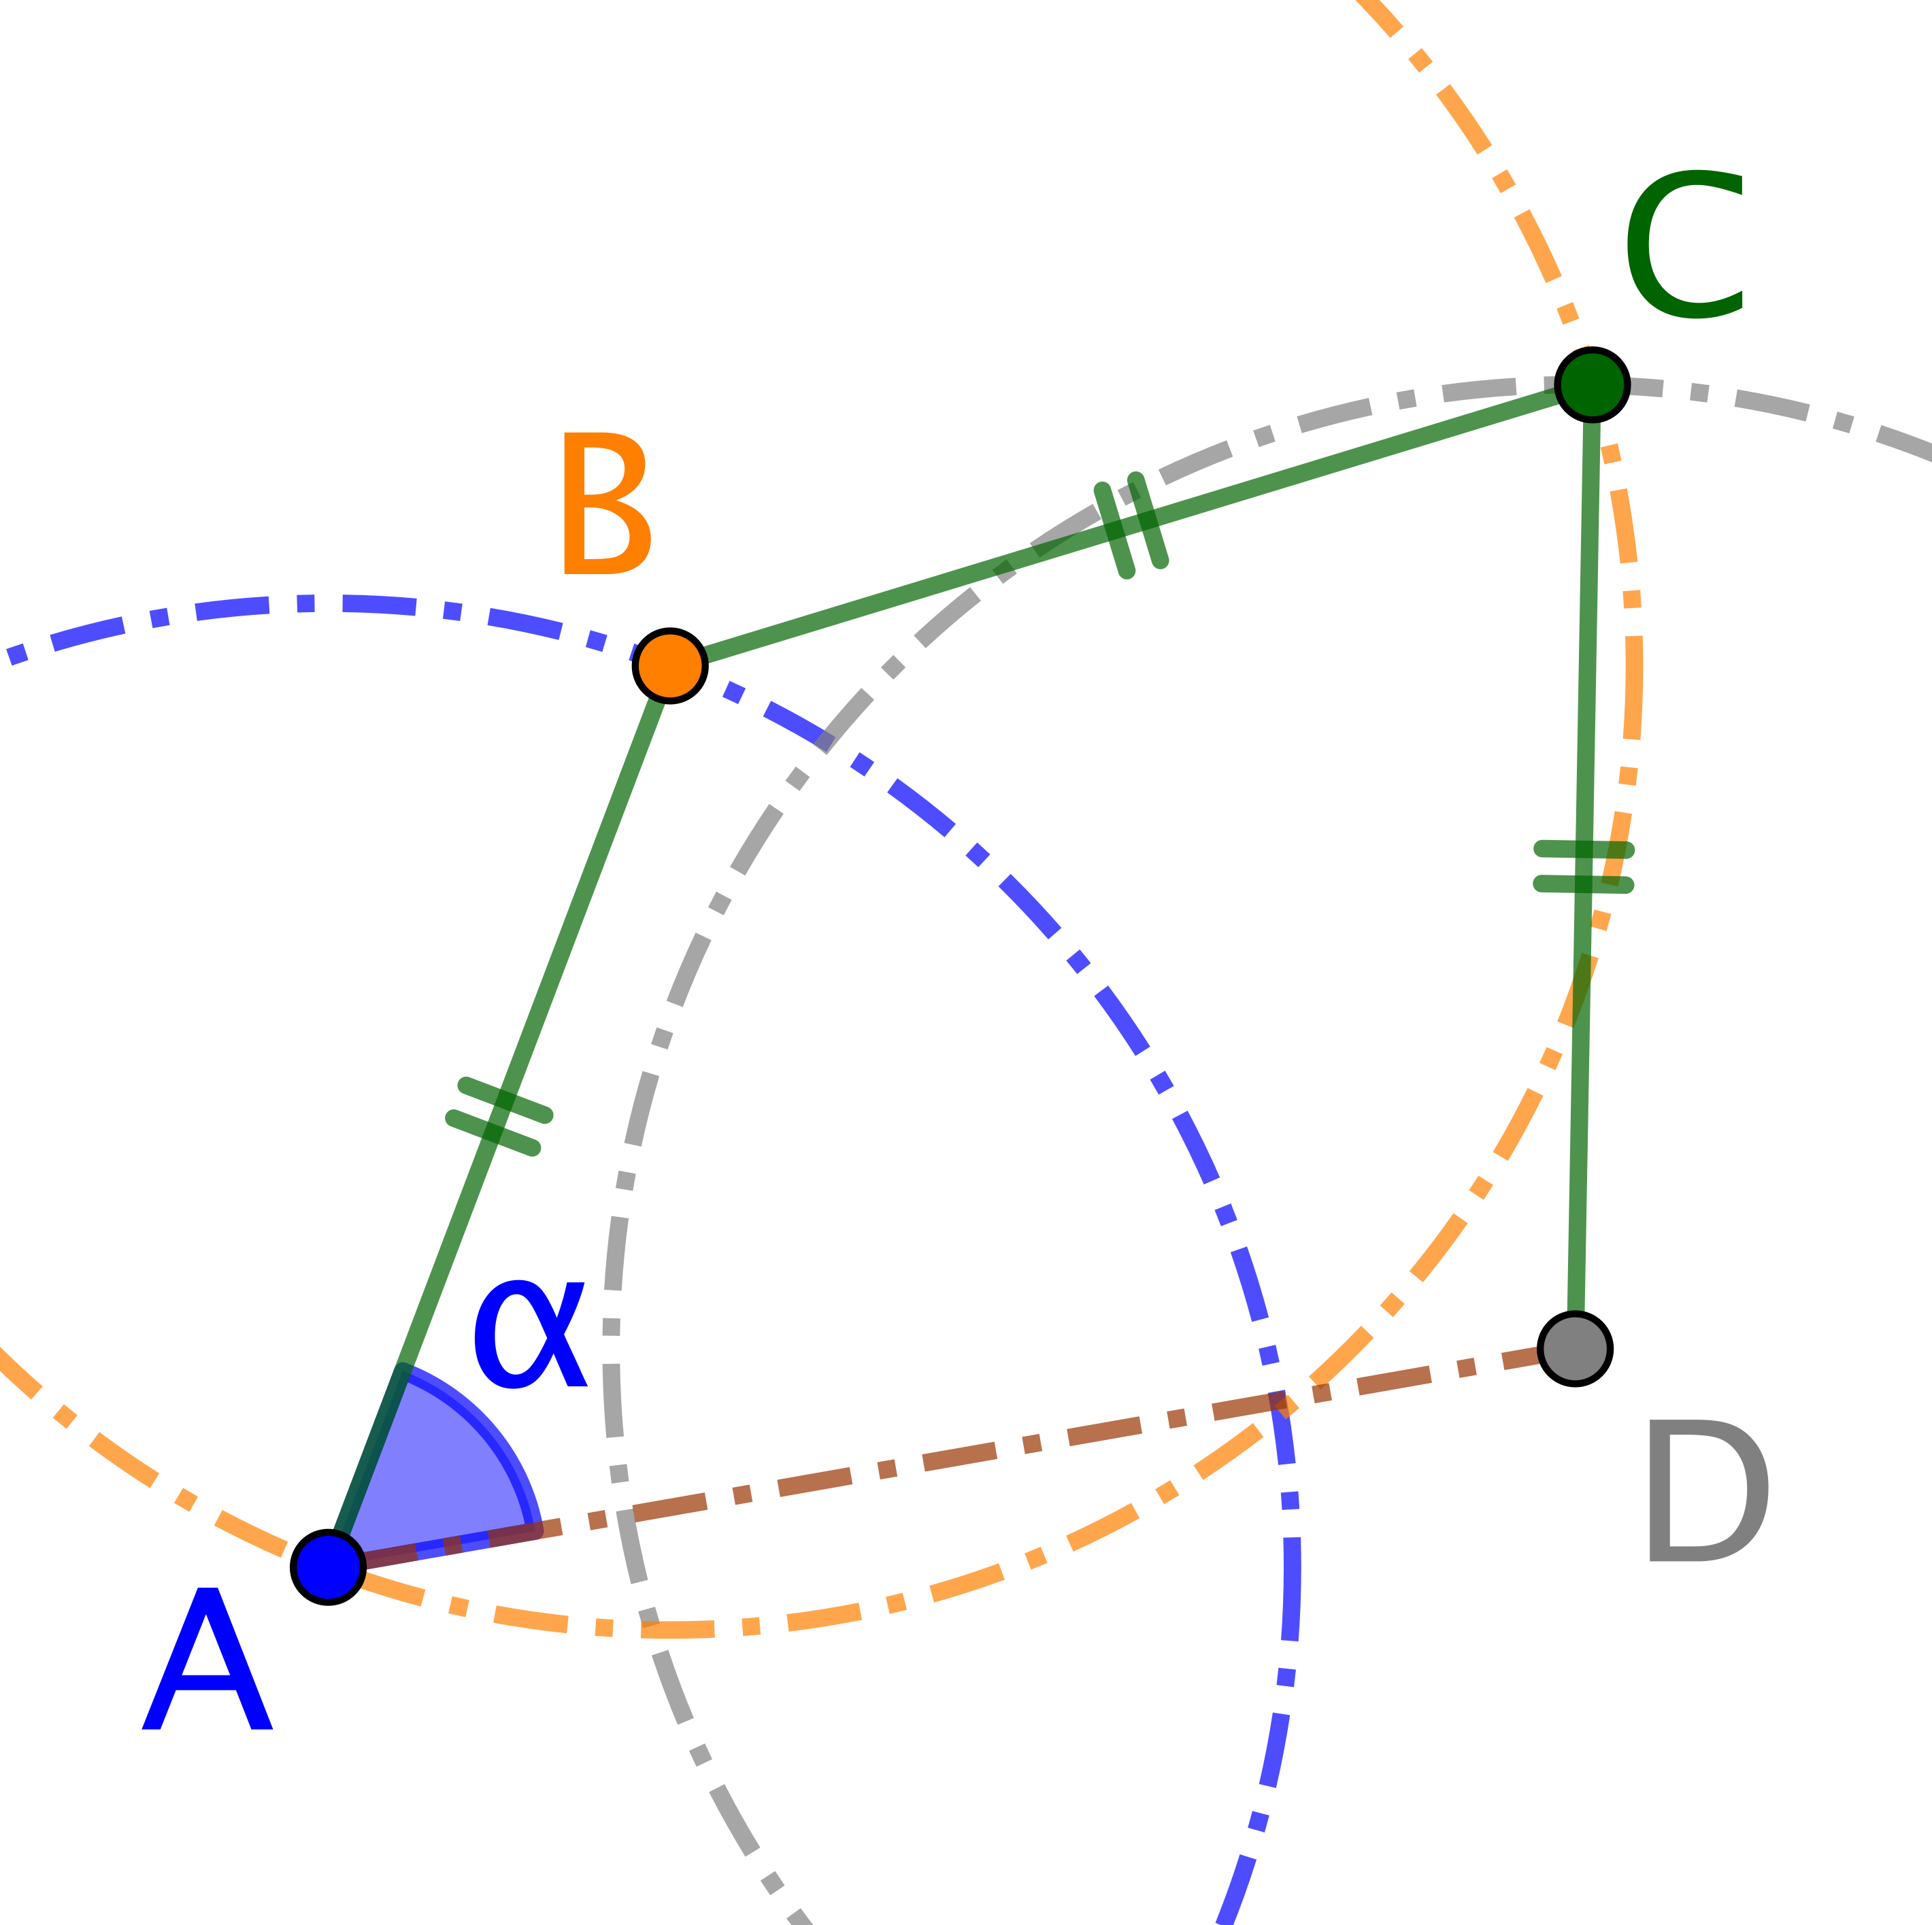
\includegraphics[scale=.4]{content/polygon/sol-must-be/2-eq-angles-circle.png}
	\end{center}

	Cherchons donc à exprimer $\area{ABCD}$ en fonction de $\alpha = \anglein{DAB}$, cet angle permettant de repérer le point mobile $B$.
	%
	\begin{itemize}
	    \item Nous avons $\alpha \in \intervalO{0}{\pi}$ et $\gamma \in \intervalO{0}{\pi}$.


	    \item Le théorème d'Al-Kashi donne
	    $BD^2 = c^2 + d^2 - 2 c d \cos \alpha$ dans le triangle $ABD$,
	    ainsi que
	    $BD^2 = 2 c^2 - 2 c^2 \cos \gamma$ dans le triangle $BCD$.
	    Donc,
	    $2 \cos \gamma = 1 - k^2 + 2 k \cos \alpha$ où l'on a posé $k = \frac{d}{c}$.
	    Notons que l'inégalité triangulaire donne $d < 3 c$, puis $0 < k < 3$.


	    \item La formule trigonométrique de l'aire d'un triangle donne
	    $\area{ABD} = \num{.5} c d \sin \alpha$
	    et
	    $\area{BCD} = \num{.5} c^2 \sin \gamma$,
	   	puis
	    $\area{ABCD} = \num{.5} c^2 ( k \sin \alpha + \sin \gamma )$,
	    de sorte que
    	$\area{ABCD} = \num{.5} c^2 f(\alpha)$
    	en posant 
    	$f(\alpha) = k \sin \alpha + \sqrt{1 - \num{.25} ( 1 - k^2 + 2 k \cos \alpha)^2}$,
	    car 
	    $\sin \gamma = \sqrt{1 - \cos^2 \gamma}$.


	    \item Passons à l'étude de $\sder{f}{1}(\alpha) = 0$, en nous souvenant que nous n'avons pas besoin d'atteindre le maximum de $f$, mais juste de pouvoir faire augmenter localement $f(\alpha)$. 
	    Dans les implications suivantes, nous avons posé 
	    $\onelist{S} = \sin \alpha$ et $\onelist{C} = \cos \alpha$.
	    
	    \begin{stepcalc}[style=ar*, ope={\implies[d'où]}]
	        \sder{f}{1}(\alpha) = 0
	    \explnext{}
	        k \onelist{C}
	        +
	        \dfrac{ k \onelist{S} ( 1 - k^2 + 2 k \onelist{C}) }{ 2 \sqrt{1 -  \num{.25} ( 1 - k^2 + 2 k \onelist{C})^2} }
	        =
	        0
	    \explnext{}
	        \onelist{S} ( 1 - k^2 + 2 k \onelist{C}) 
	        =
	        - 2 \onelist{C} \sqrt{1 - \num{.25} ( 1 - k^2 + 2 k \onelist{C})^2}
	    \explnext{}
	        \onelist{S}^2 ( 1 - k^2 + 2 k \onelist{C})^2
	        =
	        4 \onelist{C}^2 \big( 1 - \num{.25} ( 1 - k^2 + 2 k \onelist{C})^2 \big)
	    \explnext{}
	        ( 1 - k^2 + 2 k \onelist{C})^2 (\onelist{S}^2 + \onelist{C}^2)
	        =
	        4 \onelist{C}^2
	    \explnext*{$\onelist{C}^2 + \onelist{S}^2 = 1$}{}
	        ( 1 - k^2 + 2 k \onelist{C})^2 - 4 \onelist{C}^2 = 0
	    \explnext{}
	        ( 1 - k^2 + 2 k \onelist{C} - 2 \onelist{C} )
	        \,
	        ( 1 - k^2 + 2 k \onelist{C} + 2 \onelist{C} )
	        = 0
	    \explnext{}
	        (1 - k) ( 1 + k - 2 \onelist{C} )
	        \,
	        (1 + k) ( 1 - k + 2 \onelist{C} ) = 0
	    \explnext*{$k > 0$}{}
	        k = 1
	        \,\, \text{ou} \,\,
	        \onelist{C} \in \setgene{ \frac{k - 1}{2} , \frac{k + 1}{2} }
	    \end{stepcalc}


	    \item $k = 1$ signifie que $ABCD$ est un losange, non rectangle, car $\anglein{ABC} \neq \anglein{BCD}$.
	    Dans ce cas, en bougeant un peu le sommet $B$ parallèlement à $(AD)$, tout en faisant
	    augmenter $\alpha$ légèrement si $\alpha \in \intervalO{0}{\frac{\pi}{2}}$,
	    ou
	    diminuer $\alpha$ légèrement si $\alpha \in \intervalO{\frac{\pi}{2}}{\pi}$,%
	    \footnote{
	        $B$ se déplace vers la gauche dans notre cas.
	    }
	    nous obtenons un parallélogramme de même aire, mais de périmètre diminué.%
	    \footnote{
	        Si besoin, se reporter à la preuve du fait \ref{iso-para}.
	    }
	    On obtient au final un \ngone\ convexe $\primeit{\setproba{P}}$ tel que
		$\perim{\primeit{\setproba{P}}} < \perim{\setproba{P}}$
		et
		$\area{\primeit{\setproba{P}}} = \area{\setproba{P}}$,
		qu'il suffit d'agrandir pour conclure.


	    \item Pour $k \neq 1$ et $\onelist{C} = \frac{k - 1}{2}$,
	    nous avons $2\cos \alpha = k - 1$, 
	    puis 
	    $2 \cos \gamma = 1 - k^2 + k(k - 1) = 1 - k$,
	    soit
	    $\cos \gamma = - \cos \alpha$ qui fournit
	    $\gamma = \pi - \alpha$, en se souvenant que $(\alpha , \gamma) \in \intervalO{0}{\pi}^2$.
	    Notons que $\alpha \neq \frac{\pi}{2}$ et $\gamma \neq \frac{\pi}{2}$, car $k \neq 1$.
	    %
	    
	    
	    XXX


	    \item Pour $k \neq 1$ et $\onelist{C} = \frac{k + 1}{2}$,
	    comme au début du point précédent,
	    nous avons $\cos \gamma = \cos \alpha$, puis $\gamma = \alpha$ avec $(\alpha , \gamma) \in \intervalO{0}{\pi}^2$.
	    Notons qu'ici $0 < k < 1$, puis $(\alpha , \gamma) \in \intervalO{0}{\frac{\pi}{3}}^2$.
	    Dès lors, les monotonies de $\sin$ et $\cos$ sur $\intervalO{0}{\frac{\pi}{3}}$, combinées à $1 - k^2 + 2 k \cos \alpha \geq 0$, impliquent la stricte croissance de $f$ sur $\intervalO{0}{\frac{\pi}{3}}$.%
	    \footnote{
	    	Nous utilisons la composition de fonctions monotones, ce qui n'est pas toujours faisable.
	    }
	    Il suffit donc d'augmenter légèrement la valeur de  $\alpha$.
	\end{itemize}
	
	\null\vspace{-6ex}
\end{proof}


\begin{remark}
    Ce qui précède donne envie de faire appel à la méthode des extrema liés pour plus d'élégance dans les calculs.
    Étudions donc les extrema de
	$f(\alpha , \gamma) = k \sin \alpha + \sin \gamma$
	sur $\intervalO{0}{\pi}^2$ sous la contrainte
	$g(\alpha , \gamma) = 0$
	avec
	$g(\alpha , \gamma) = 1 - k^2 + 2 k \cos \alpha - 2 \cos \gamma$.
	%
    Si un extremum existe, alors nous avons $\lambda \in \RR$ tel que
    $\pder[i]{f}{\alpha}{1} = \lambda \pder[i]{g}{\alpha}{1}$
	et
    $\pder[i]{f}{\gamma}{1} = \lambda \pder[i]{g}{\gamma}{1}$,
	de sorte que
	$k \cos \alpha = - 2 k \lambda \sin \alpha$,
	soit
	$\cos \alpha = - 2 \lambda \sin \alpha$,
	et aussi
	$\cos \gamma = 2 \lambda \sin \gamma$.
	Nous avons alors les deux alternatives suivantes qui rejoignent les arguments de la preuve précédente.
	%
	\begin{enumerate}
	    \item Si $\lambda = 0$,
	    alors
	    $\alpha = \gamma = \frac{\pi}{2}$, puis $k = 1$. 

	    \item Si $\lambda \neq 0$,
	    alors
	    $\cos \alpha \sin \gamma = - \cos \gamma \sin \alpha$,
	    puis
	    $\sin (\alpha + \gamma) = 0$,
	    et
	    $\gamma = \pi - \alpha$.
	\end{enumerate}
\end{remark}


\begin{remark}
	Une démonstration géométrique du fait \ref{must-be-iso} est possible via un résultat attribué à Zénodore%
	\footnote{
	    La preuve du résultat de Zénodore est un peu fastidieuse.
	}
	sur la maximisation de l'aire totale de deux triangles isocèles de bases fixées, et de périmètre total constant:
	ce résultat affirme que les deux triangles doivent avoir des angles en leur sommet principal de même mesure.
	Malheureusement, cette preuve échoue lors de la disparition d'un sommet en choisissant la paire optimale de triangles isocèles pour construire un nouveau \ngone\ \focus{plus gros}.
\end{remark}


% ----------------------- %


\begin{fact} \label{must-be-reg}
	Si un \ngone\ $\setproba{P}$ n'est pas un \nreg\ convexe,
	alors il existe un \ngone\ convexe $\primeit{\setproba{P}}$ tel que
	$\perim{\primeit{\setproba{P}}} = \perim{\setproba{P}}$
	et
	$\area{\primeit{\setproba{P}}} > \area{\setproba{P}}$.
\end{fact}


\begin{proof}
	Il suffit d'utiliser les faits \ref{must-be-conv}, \ref{must-be-equi} et \ref{must-be-iso}.
\end{proof}


% ----------------------- %


Pour en finir avec le problème d'isopérimétrie polygonal, nous aurons besoin du fait suivant.


\begin{fact} \label{nregs-sorting}
	Si $\setproba*{R}{1}$ et $\setproba*{R}{2}$ sont respectivement un \xgone{k_1} et un \xgone{k_2}, tous les deux réguliers convexes, avec 
	$k_1 < k_2$ et $\perim{\setproba*{R}{1}} = \perim{\setproba*{R}{2}}$,
	alors
	$\area{\setproba*{R}{1}} < \area{\setproba*{R}{2}}$.
\end{fact}


\begin{proof}
    Il est connu, et facile à démontrer, qu'un \nreg\ convexe $\setproba{R}$ vérifie
    $\perim{\setproba{R}} = 2 n \sin (\frac{\pi}{n}) \rho$
    et
	$\area{\setproba{R}} = n \sin (\frac{\pi}{n})  \cos (\frac{\pi}{n}) \rho^2$
	où $\rho$ désigne le rayon du cercle circonscrit à $\setproba{R}$.
	Ceci donne 
	$\area{\setproba{R}} = \frac{\perim{\setproba{R}}^2}{4 n \tan (\frac{\pi}{n})}$,
	puis amène à justifier que 
	$k_1 \tan (\frac{\pi}{k_1}) > k_2 \tan (\frac{\pi}{k_2})$,
	c'est-à-dire que la suite $\big( k \tan (\frac{\pi}{k}) \big)_{k \in \NN_{\geq 3}}$ est strictement décroissante.
	
	
	XXXX
\end{proof}

